\documentclass[12pt]{article}
\usepackage[margin=1in]{geometry}
\usepackage{amsmath,amssymb,physics}
\usepackage{siunitx}
\usepackage{graphicx}
\usepackage{booktabs}
\usepackage{caption}
\usepackage{hyperref}
\usepackage[nameinlink]{cleveref}
\usepackage{datetime2}
\usepackage{placeins} 
\sisetup{separate-uncertainty = true, detect-all = true}
\graphicspath{{fig/}}

% ---------- Metadata ----------
\newcommand{\ExpTitle}{Lab 2: Capacitance}
\newcommand{\YourName}{Zemon Xiao}
\newcommand{\YourPartner}{Yifan Li}
\newcommand{\Course}{PHYS-142}
\newcommand{\LabDate}{\DTMdisplaydate{2025}{10}{14}{-1}}
\newcommand{\ManualTitle}{Lab 2: Capacitance}


\newcommand{\Avalue}{2.46\times 10^{-2}} % m^2
\newcommand{\epsvalue}{8.85\times 10^{-12}} % F/m

\begin{document}

\begin{center}
    {\LARGE \textbf{\ExpTitle}}\\[6pt]
    {\large \Course}\\[4pt]
    \textbf{Author:} \YourName \quad
    \textbf{Partner:} \YourPartner \\
    \textbf{Date:} \LabDate
\end{center}

\begin{abstract}
The purpose of this experiment was to investigate how the capacitance of a parallel-plate capacitor depends on plate separation and to examine the effect of inserting dielectric materials between the plates.  We used a variable parallel-plate capacitor connected to an electrometer and a \SI{30}{V} electrostatic voltage source, recording the voltage as the plate spacing varied from \SI{0.3}{cm} to \SI{8.0}{cm}.  The effective system capacitance was modeled as \(C_{\text{total}}=\kappa\varepsilon_{0}A/d+C_{\mathrm{sys}}\).  Using limiting-case analysis, the stored charge and parasitic capacitance were found to be
\(Q=(1.34\pm0.03)\times10^{-9}\,\mathrm{C}\) and
\(C_{\mathrm{sys}}=(3.24\pm0.14)\times10^{-11}\,\mathrm{F}\).
Additional tests with paper, plastic, and glass dielectrics at fixed charge yielded mean dielectric constants of
\(\kappa_{\text{paper}}\approx1.1\),
\(\kappa_{\text{plastic}}\approx4.7\),
and
\(\kappa_{\text{glass}}\approx0.8\),
demonstrating the qualitative validity of the relation \(V_{\mathrm{in}}=V_{\mathrm{out}}/\kappa\) but also highlighting the influence of leakage and drift.  Within experimental uncertainty, the measured \(V(d)\) relationship agrees with the theoretical model incorporating the system capacitance term.
\end{abstract}

% ---------------- THEORY ----------------
\section{Theory}
A capacitor stores equal and opposite charges on two conductors separated by an insulator.  The capacitance is defined by
\begin{equation}
    C=\frac{Q}{V}.
    \label{eq:def}
\end{equation}
For a parallel-plate geometry with plate area \(A\) and separation \(d\), Gauss’s law gives \(E=\sigma/\varepsilon_0\) and
\begin{equation}
    V=Ed=\frac{Qd}{\varepsilon_0A}\quad\Rightarrow\quad C_0=\frac{\varepsilon_0A}{d}.
    \label{eq:cpp_vac}
\end{equation}
Filling the gap with a dielectric of relative permittivity \(\kappa\) yields
\begin{equation}
    C=\kappa C_0=\kappa\frac{\varepsilon_0A}{d}.
    \label{eq:cpp_die}
\end{equation}
The real apparatus includes a separation-independent parasitic capacitance \(C_{\mathrm{sys}}\) from the electrometer and leads, so the effective capacitance is
\begin{equation}
    C_{\text{total}}(d)=\kappa\frac{\varepsilon_0A}{d}+C_{\mathrm{sys}}.
    \label{eq:ctotal}
\end{equation}
Charging and then isolating the system makes \(Q\) approximately constant. Combining \cref{eq:def,eq:ctotal} gives the working model
\begin{equation}
    V(d)=\frac{Q}{\kappa\varepsilon_0A/d+C_{\mathrm{sys}}}.
    \label{eq:vd_model}
\end{equation}
For small \(d\), \(V\simeq Qd/(\kappa\varepsilon_0A)\) (linear in \(d\)); for large \(d\), \(V\simeq Q/C_{\mathrm{sys}}\) (plateau). If a dielectric is inserted at fixed \(Q\), then
\begin{equation}
    Q=C_0V_0=\kappa C_0V\quad\Rightarrow\quad V=\frac{V_0}{\kappa},
    \qquad \kappa=\frac{V_{\text{out}}}{V_{\text{in}}}\,.
    \label{eq:ratio_kappa}
\end{equation}

% ---------------- PROCEDURE ----------------
\section{Experimental Procedure}
We used a basic electrometer, a variable parallel-plate capacitor, a \SI{30}{V} electrostatic voltage source, the PASCO 850 Universal Interface, and dielectric samples of paper, plastic, and glass.  The plates were adjusted to be parallel with an initial separation of approximately \SI{0.2}{cm}, verified visually from both top and side views.  The fixed plate was connected to ground and the movable plate to the electrometer input through a twin-lead cable kept clear of the body to minimize stray capacitance.  The electrometer output was linked to the 850 interface and Capstone software configured for a user-entered separation (in centimeters) and a measured voltage channel.

For the plate-separation study, the electrometer was set to the \SI{100}{V} range and zeroed after discharging the plates by contact.  The capacitor was charged momentarily through the \SI{+30}{V} terminal and then left electrically isolated so that the total charge remained approximately constant.  We then measured the voltage as the plate separation was varied between \SI{0.3}{cm} and \SI{8.0}{cm}.  One experimenter operated the computer while the other adjusted the plate position, and all others remained at least half a meter away to reduce coupling.  Each voltage was recorded using the “Keep Sample’’ function in Capstone, producing a complete data set of voltage versus distance.  The entire sequence was repeated to ensure reproducibility.

To study the dielectric effect, the plates were fixed at \SI{8}{cm}.  The capacitor was again charged to \SI{30}{V} and isolated.  Alternate voltage readings were taken with and without each dielectric inserted between the plates.  For paper, approximately ten sheets were stacked and lowered vertically into the gap without touching the plates while the operator’s other hand remained on the electrometer signal terminal to drain static charge.  For plastic and glass, framed samples were used to minimize handling and prevent damage.  Multiple out/in cycles were recorded for each material to allow averaging and estimation of the uncertainty.
\begin{figure}[htbp]
  \centering
  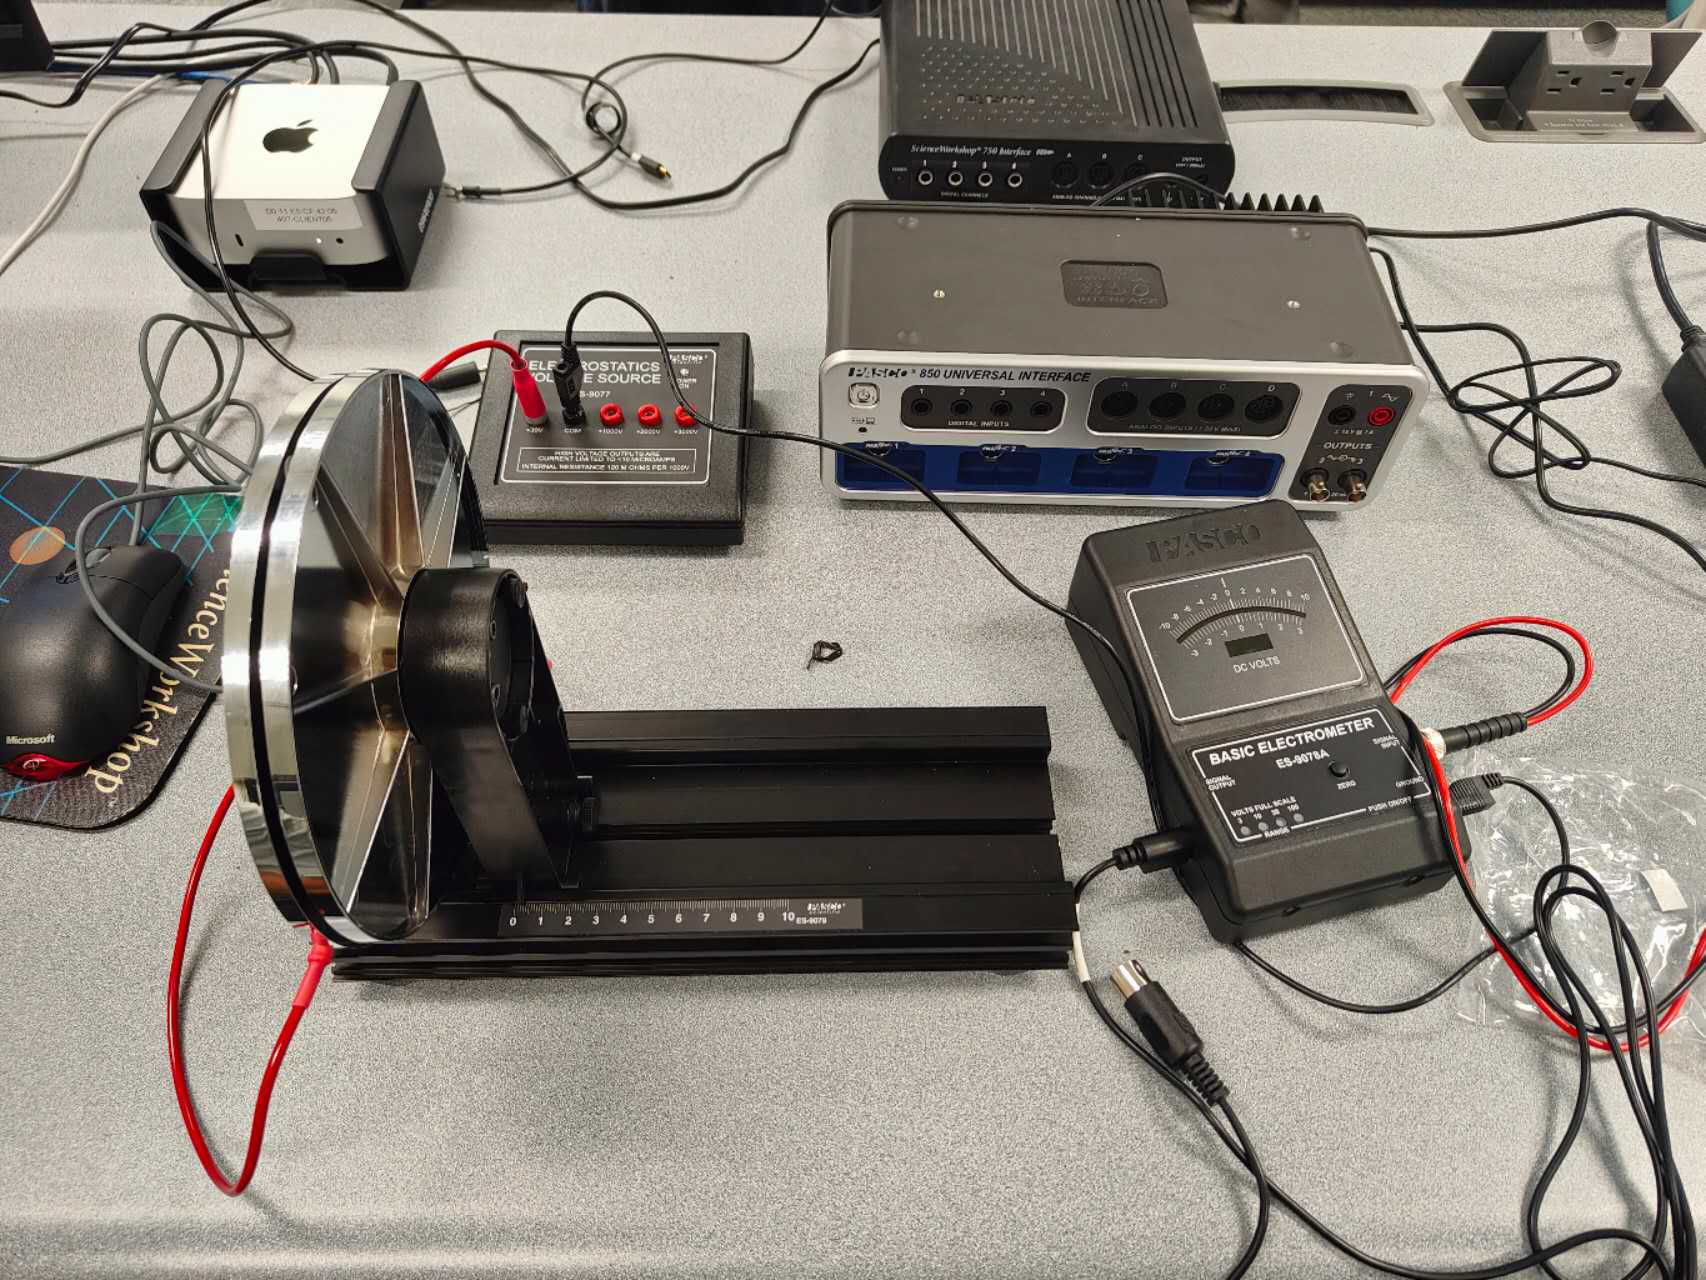
\includegraphics[width=0.9\linewidth]{1.jpg}
  \caption{Photograph of the experimental apparatus. The variable parallel–plate capacitor is connected to the electrometer via short leads; the fixed plate is grounded and the movable plate goes to the electrometer input. The PASCO 850 interface and \SI{30}{V} source are placed away from the plates to reduce stray capacitance.}
  \label{fig:apparatus}
\end{figure}


% ---------------- DATA ANALYSIS ----------------
\newpage
\section{Data Analysis}

\subsection*{Part A: Voltage--distance relation}

We first examine the raw voltage--distance records from two independent runs. Both runs display a monotonic increase in \(V\) with \(d\), consistent with the decrease of the parallel-plate term \(\kappa\varepsilon_0A/d\) as the plates are separated. The independent data sets are shown in \cref{fig:run1,fig:run2}. To quantify reproducibility, we compute, at each separation, the mean voltage and the inter-run standard deviation as an estimate of random uncertainty. The combined mean series with one–standard–deviation error bars is presented in \cref{fig:combined}. We compare this combined series to the model
\begin{equation}
    V(d)=\frac{Q}{\kappa\varepsilon_0A/d + C_{\mathrm{sys}}}\,,
    \label{eq:vd_model_analysis}
\end{equation}
and display the residuals \(V_{\text{data}}-V_{\text{model}}\) in \cref{fig:resid}; finally, we propagate parameter uncertainties to obtain a parametric \(\pm1\sigma\) band in \cref{fig:band}.

\begin{figure}[htbp]
\centering
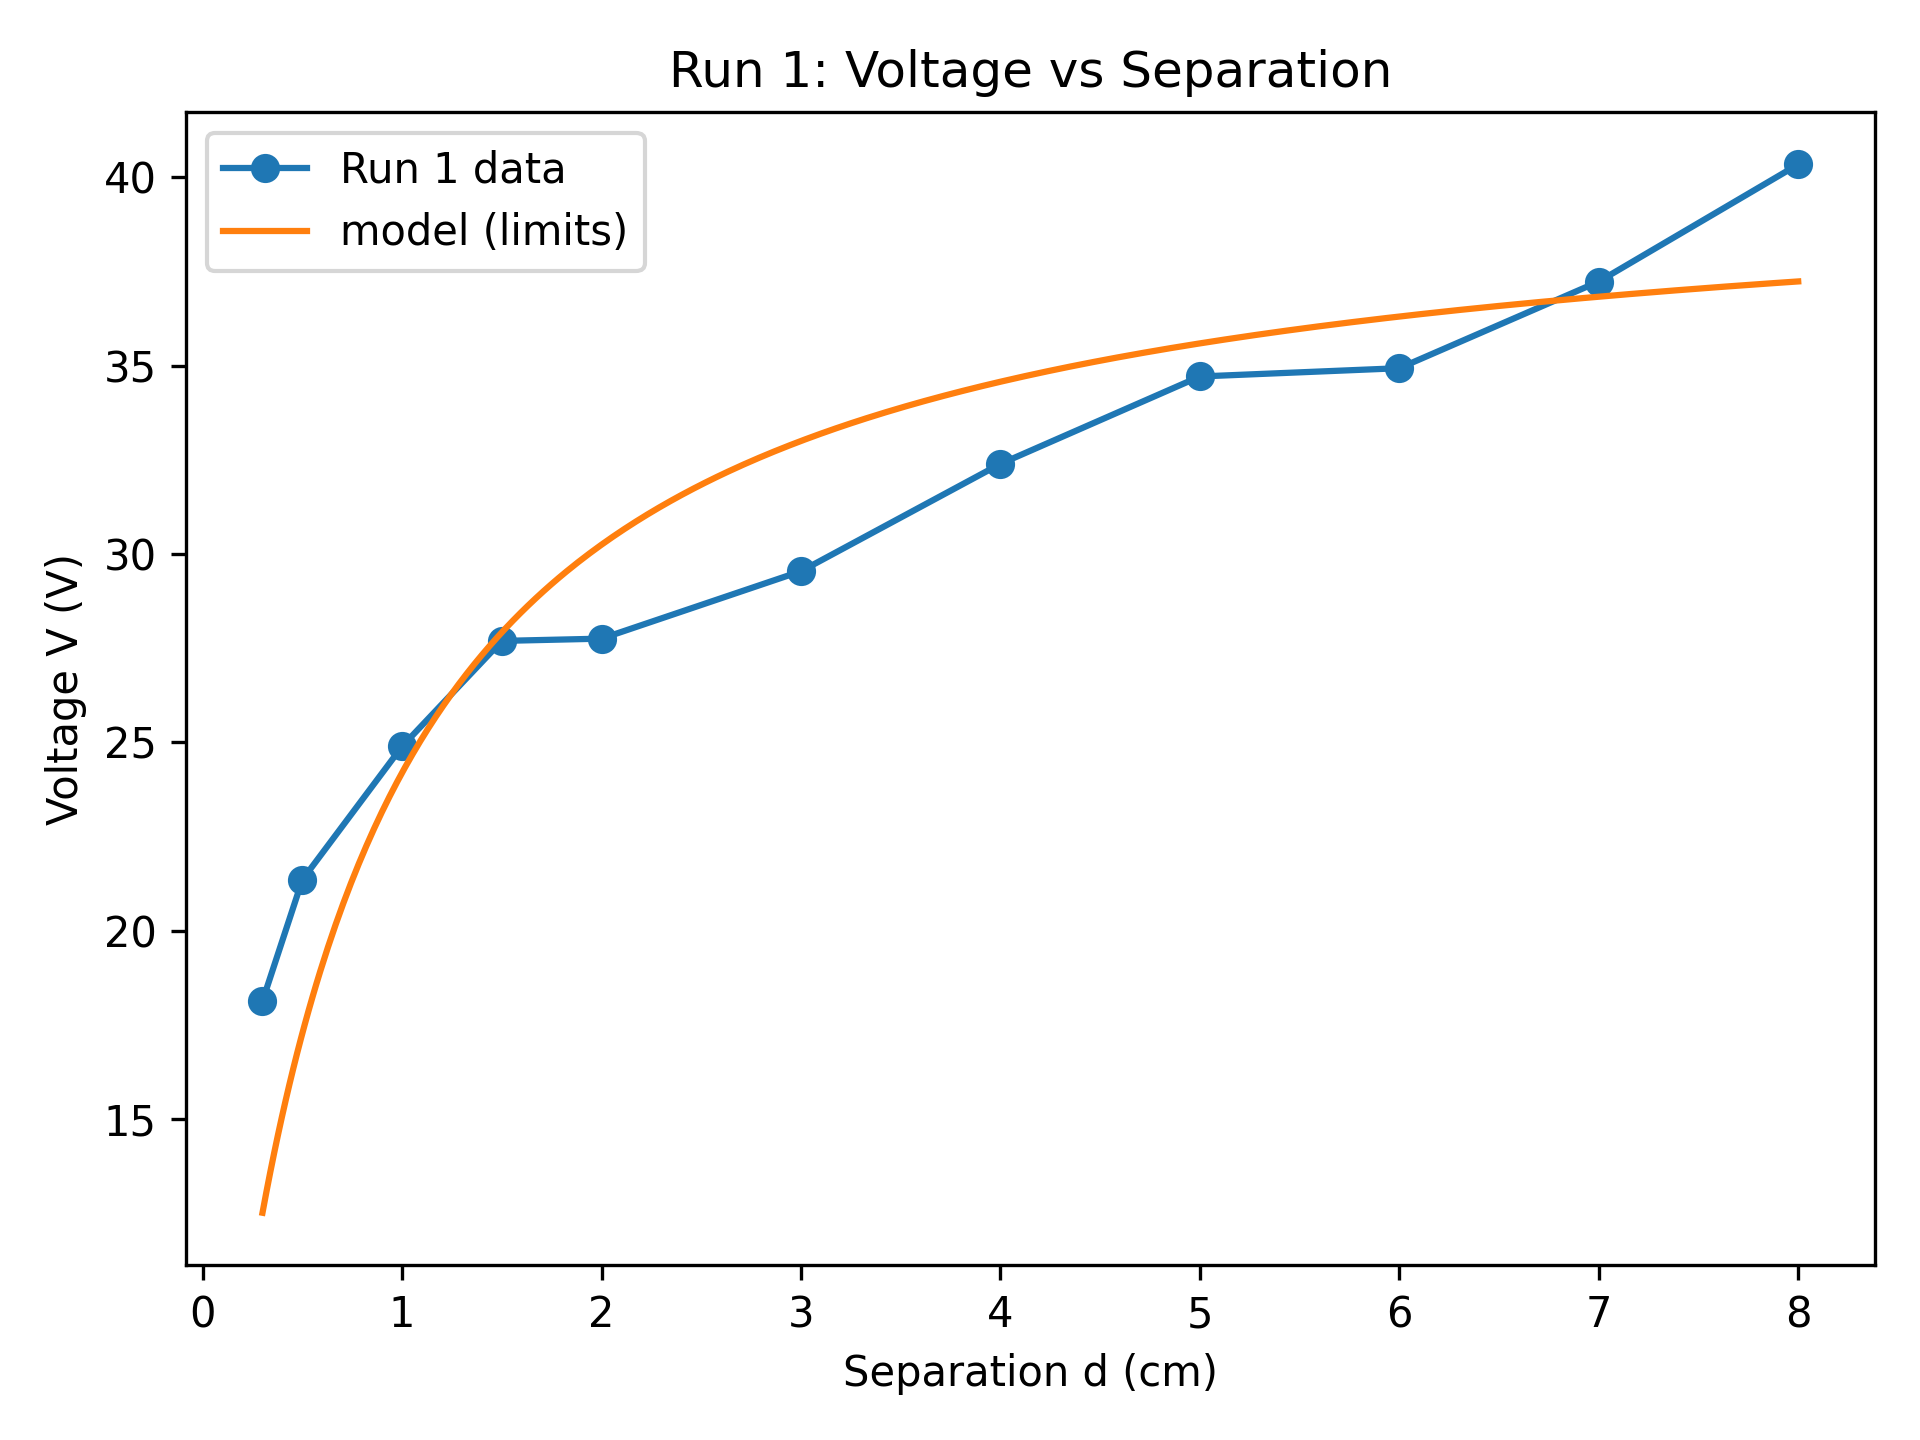
\includegraphics[width=0.82\linewidth]{PartA_Run1.png}
\caption{\textbf{Part A -- Run 1.} Voltage vs.\ separation; solid curve is \cref{eq:vd_model_analysis} evaluated with endpoint parameters from this run.}
\label{fig:run1}
\end{figure}
\FloatBarrier

\begin{figure}[htbp]
\centering
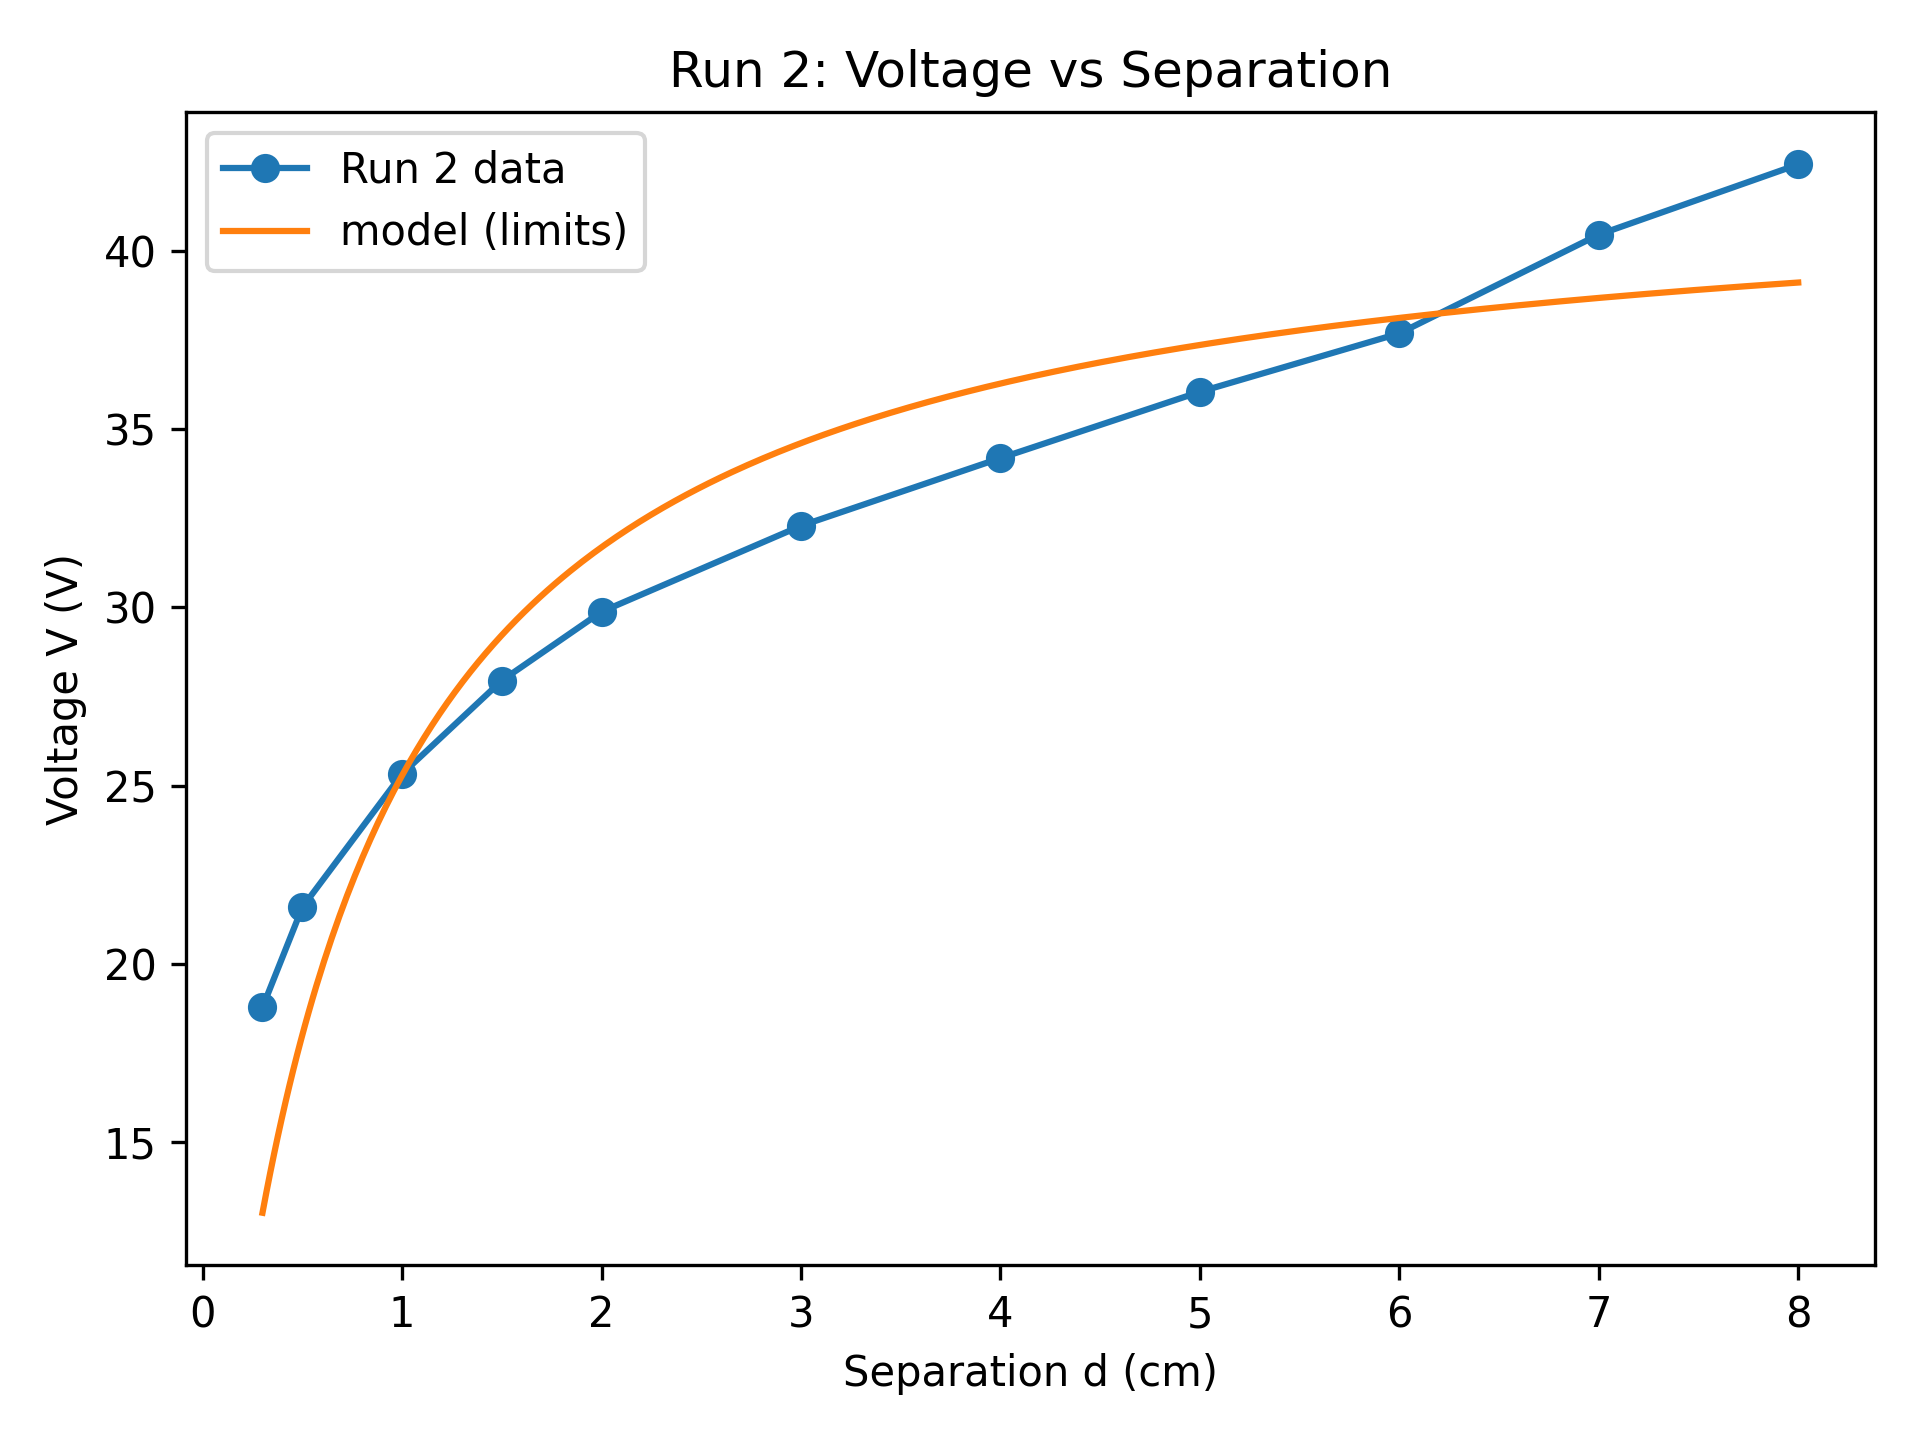
\includegraphics[width=0.82\linewidth]{PartA_Run2.png}
\caption{\textbf{Part A -- Run 2.} Independent repetition exhibiting the same rising trend, indicating reproducibility.}
\label{fig:run2}
\end{figure}
\FloatBarrier

\begin{figure}[htbp]
\centering
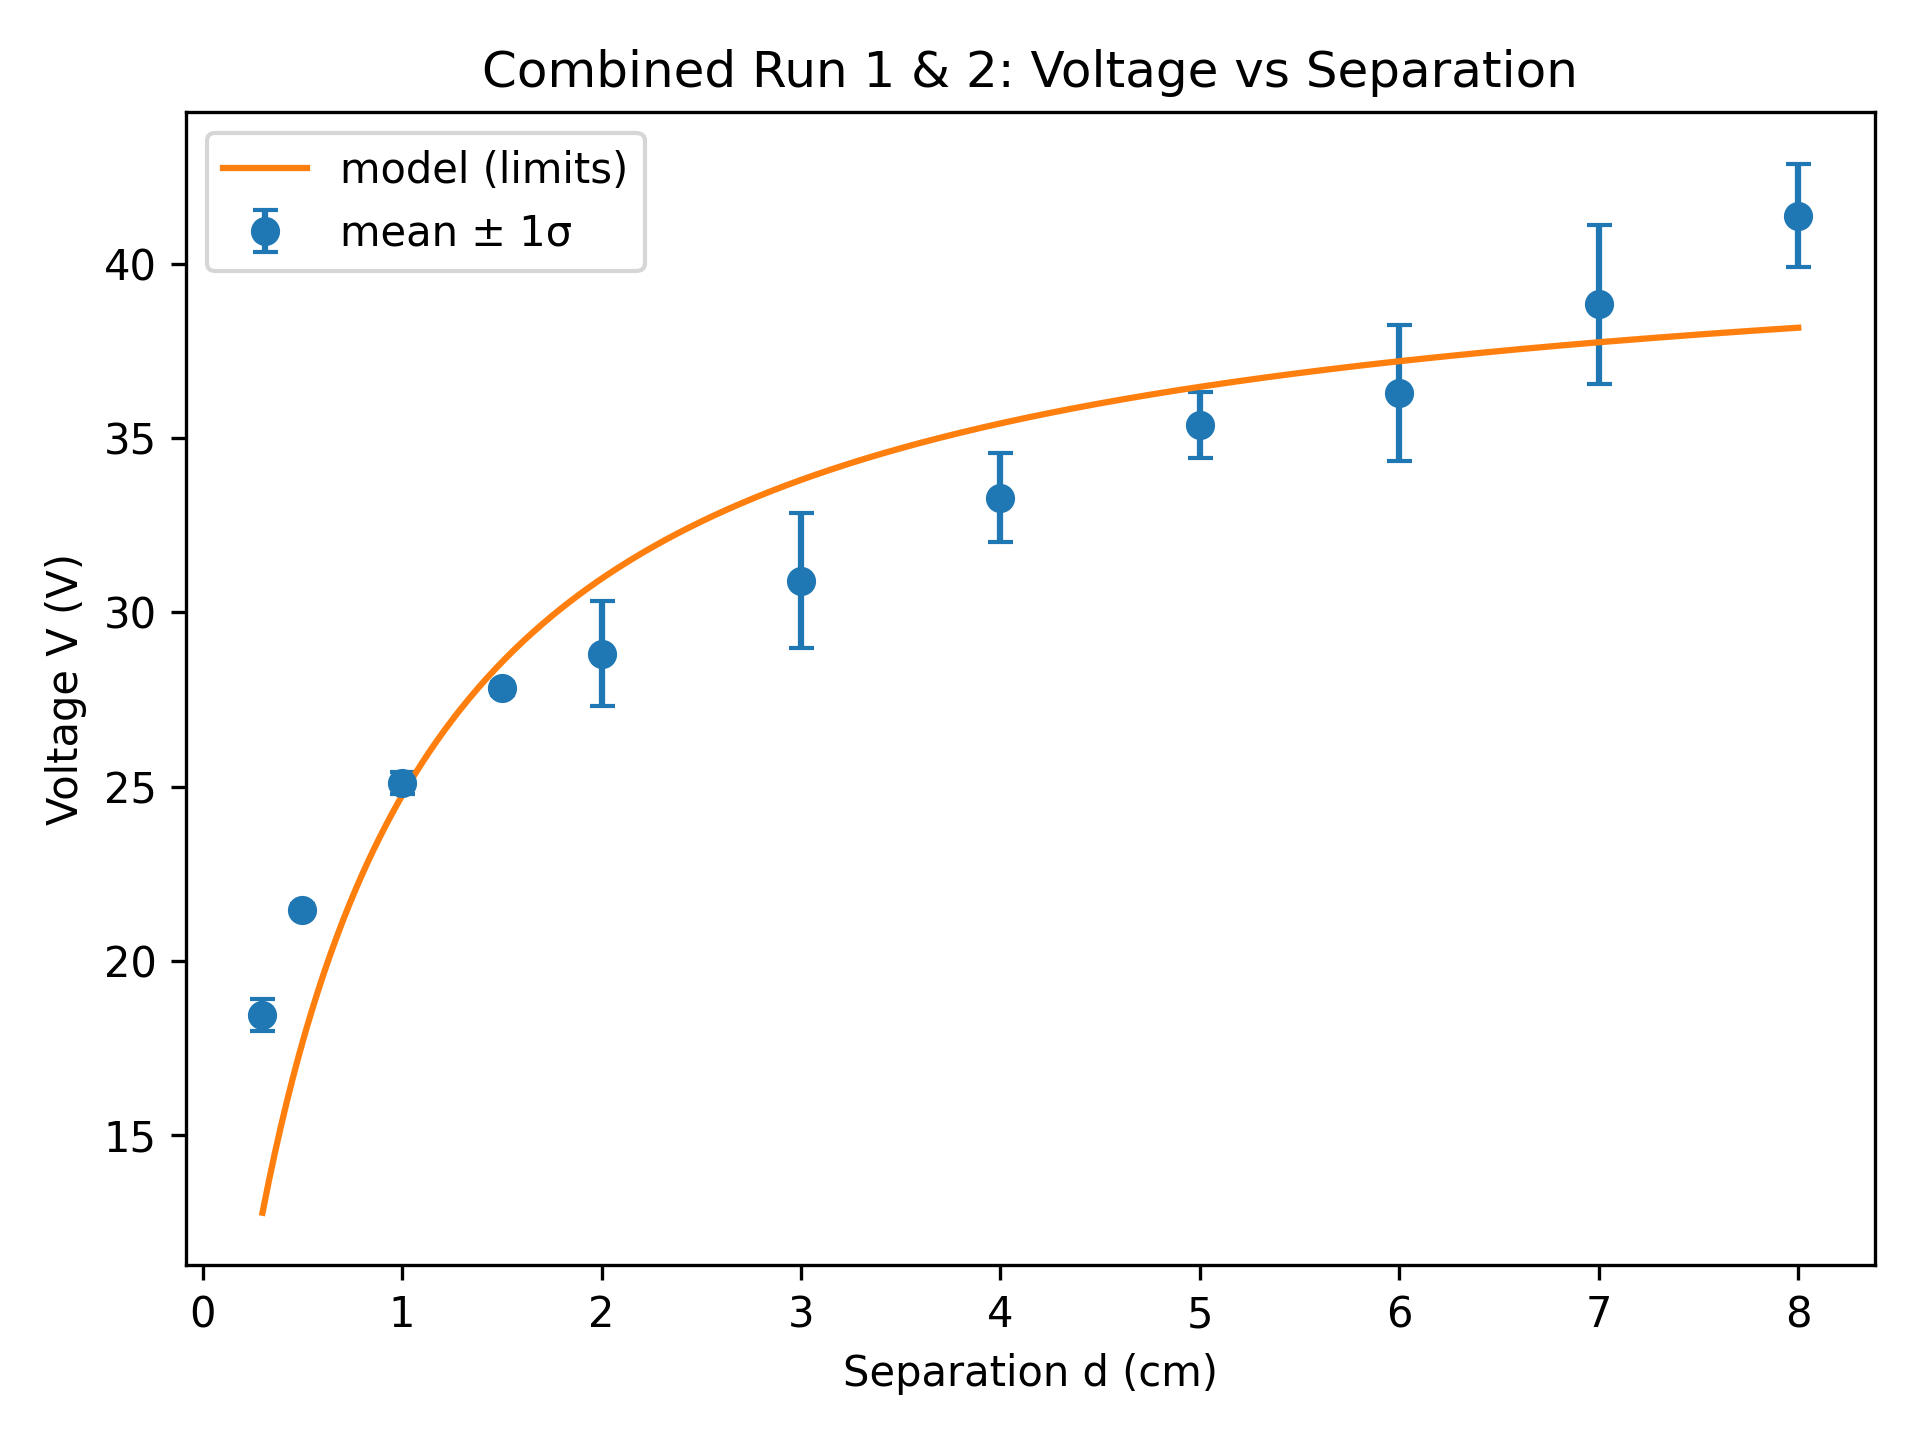
\includegraphics[width=0.82\linewidth]{PartA_Combined.png}
\caption{\textbf{Part A -- Combined mean \(\pm\) SD.} Average of Run~1 and Run~2 with inter-run standard-deviation error bars. The curve is the model in \cref{eq:vd_model_analysis} with parameters estimated from limiting cases.}
\label{fig:combined}
\end{figure}

\begin{figure}[htbp]
\centering
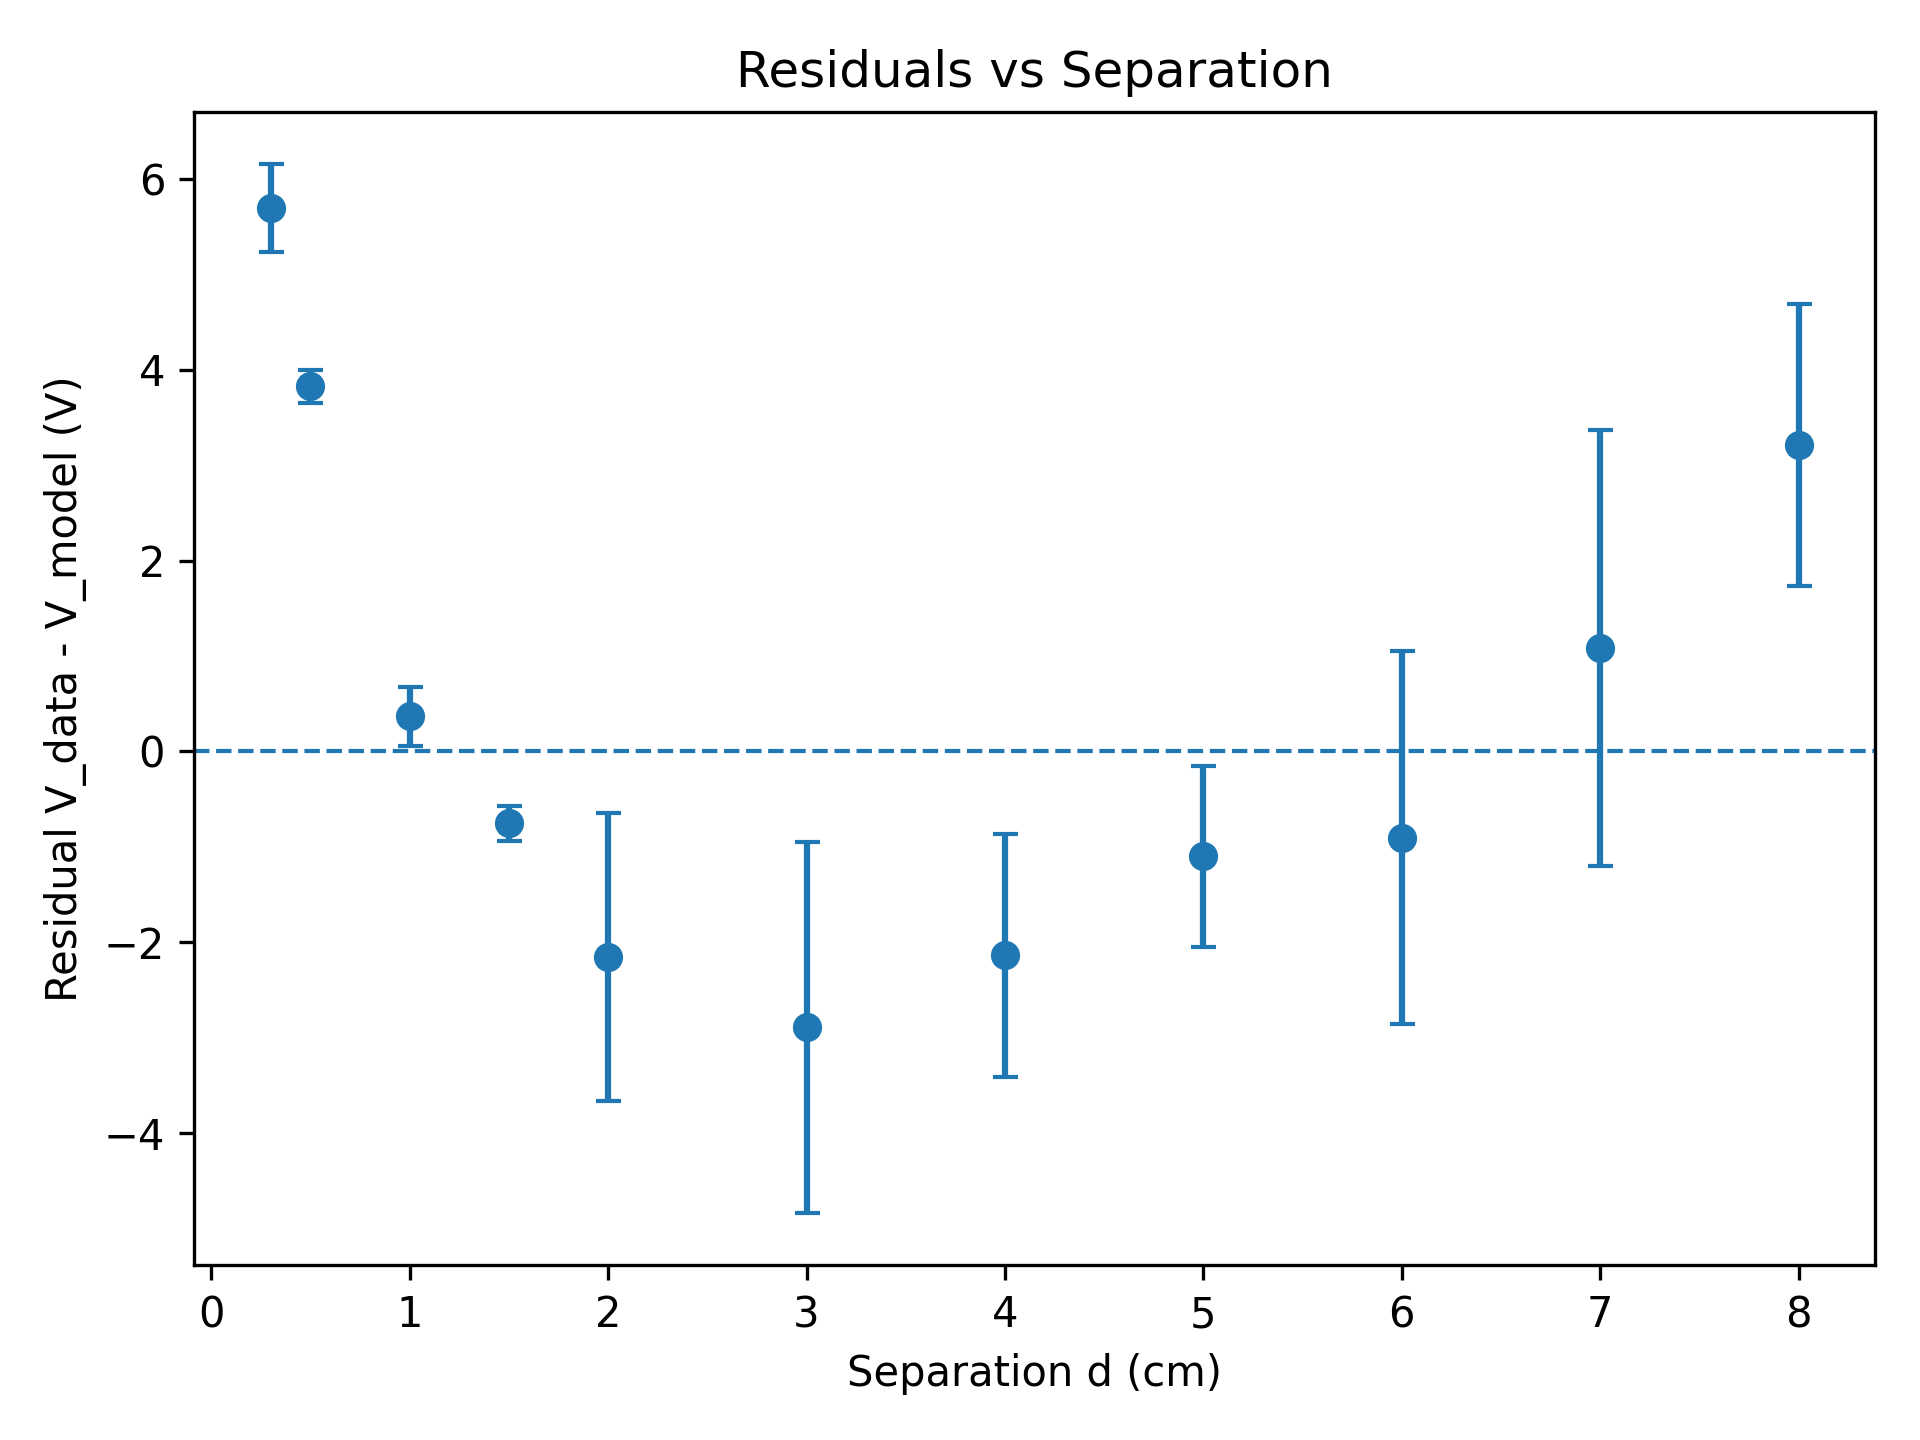
\includegraphics[width=0.82\linewidth]{PartA_residuals.png}
\caption{\textbf{Part A -- Residuals.} Difference \(V_{\text{data}}-V_{\text{model}}\) for the combined series; error bars are the inter-run SD. The absence of structure supports model adequacy within precision.}
\label{fig:resid}
\end{figure}

\paragraph{Worked example: extracting \(Q\) and \(C_{\mathrm{sys}}\) with uncertainties.}
Following the manual’s limiting-case prescription, we use the combined mean at the smallest gap \(d_{0.3}=\SI{0.003}{m}\) and at the largest gap \(d_{8.0}=\SI{0.08}{m}\). With air \((\kappa=1.00)\), \(\varepsilon_0=\num{8.85e-12}\ \si{F.m^{-1}}\) and \(A=\num{2.46e-2}\ \si{m^2}\), the geometric factor is
\begin{equation}
    \kappa\varepsilon_0A = (1.00)\times(\num{8.85e-12})\times(\num{2.46e-2})
    = \num{2.18e-13}\ \si{F\cdot m}.
    \label{eq:geom_factor}
\end{equation}
Using the combined mean voltage at the smallest gap \(V_{0.3}=\SI{18.46}{V}\) (inter-run SD \(\sigma_{V,0.3}=\SI{0.46}{V}\)), the charge is
\begin{equation}
    Q \approx \frac{V_{0.3}\,\kappa\varepsilon_0A}{d_{0.3}}
      = \frac{(\SI{18.46}{V})\times(\SI{2.18e-13}{F.m})}{\SI{0.003}{m}}
      = \SI{1.34e-9}{C}.
    \label{eq:Q_eval_analysis}
\end{equation}
Treating the voltage as the dominant uncertainty,
\begin{equation}
    \sigma_Q \approx Q \frac{\sigma_{V,0.3}}{V_{0.3}}
    = (\SI{1.34e-9}{C})\frac{0.46}{18.46}
    \approx \SI{3.3e-11}{C}.
    \label{eq:dQ}
\end{equation}
At the largest gap, the model approaches \(V\approx Q/C_{\mathrm{sys}}\). Using the combined mean \(V_{8.0}=\SI{41.4}{V}\) (SD \(\sigma_{V,8.0}=\SI{1.48}{V}\)),
\begin{equation}
    C_{\mathrm{sys}} \approx \frac{Q}{V_{8.0}}
    = \frac{\SI{1.34e-9}{C}}{\SI{41.4}{V}}
    = \SI{3.24e-11}{F}.
    \label{eq:Csys_eval_analysis}
\end{equation}
Propagating uncertainties from \(\sigma_Q\) and \(\sigma_{V,8.0}\) gives
\begin{equation}
    \sigma_{C_{\mathrm{sys}}} \approx C_{\mathrm{sys}}
    \sqrt{\left(\frac{\sigma_Q}{Q}\right)^2+\left(\frac{\sigma_{V,8.0}}{V_{8.0}}\right)^2}
    \approx (\SI{3.24e-11}{F})\times 0.0435
    \approx \SI{1.4e-12}{F}.
    \label{eq:dCsys}
\end{equation}
Inserting \(\{Q, C_{\mathrm{sys}}\}\) from \cref{eq:Q_eval_analysis,eq:Csys_eval_analysis} into \cref{eq:vd_model_analysis} yields the solid curves in \cref{fig:combined}; the first-order parametric \(\pm1\sigma\) band due to \(\sigma_Q\) and \(\sigma_{C_{\mathrm{sys}}}\) is shown in \cref{fig:band}. The residuals in \cref{fig:resid} fluctuate around zero without a discernible trend, which is consistent with random scatter plus small drift.

\begin{figure}[htbp]
\centering
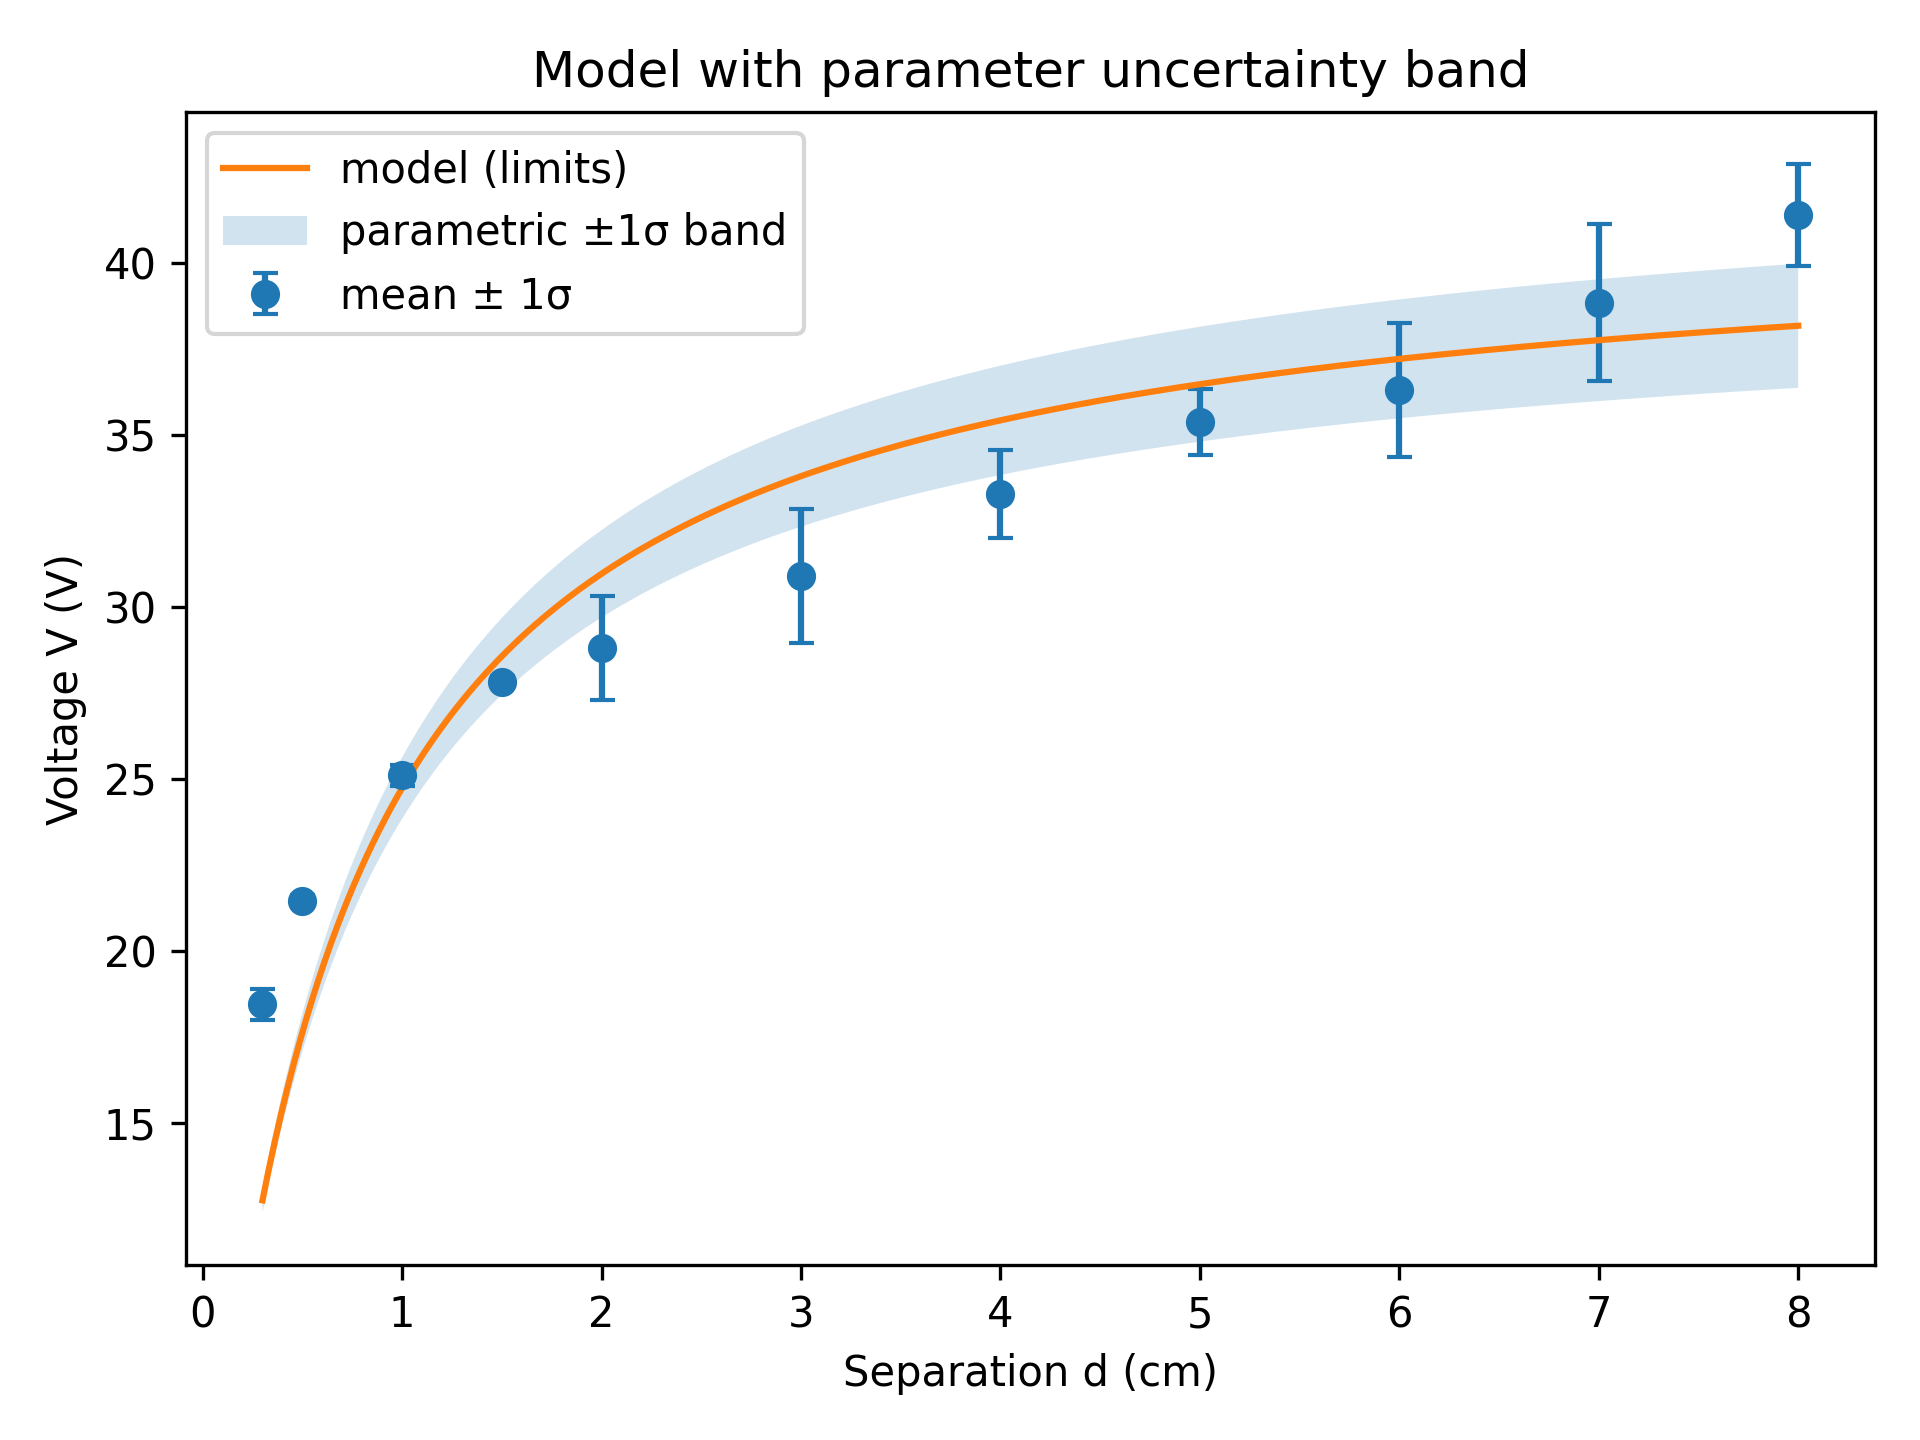
\includegraphics[width=0.82\linewidth]{PartA_params_band.png}
\caption{\textbf{Part A -- Model with parameter uncertainty band.} Shaded region shows the \(\pm1\sigma\) envelope obtained by first-order propagation of \(\sigma_Q\) and \(\sigma_{C_{\mathrm{sys}}}\).}
\label{fig:band}
\end{figure}
\FloatBarrier

\paragraph{Physical interpretation.}
Within \cref{eq:vd_model_analysis}, the initial slope \( \dv{V}{d}\big|_{d\to 0} \approx Q/(\kappa\varepsilon_0 A) \) is set by the plate geometry and the stored charge, while the large-\(d\) intercept is the plateau \(Q/C_{\mathrm{sys}}\). The agreement of both small-\(d\) and large-\(d\) limits with the data indicates that including \(C_{\mathrm{sys}}\) is essential; a pure \(1/d\) model would predict a linear \(V\)–\(d\) relation without saturation, contrary to observation.

\subsection*{Part B: Dielectric insertion at fixed \(Q\)}

For each material we alternated OUT (no sample) and IN (sample inserted) readings at fixed separation \(\SI{8}{cm}\) while the capacitor remained isolated. Denoting the OUT and IN means by \(\mu_{\text{out}}\) and \(\mu_{\text{in}}\) and their standard deviations by \(\sigma_{\text{out}}\) and \(\sigma_{\text{in}}\), the dielectric constant follows from charge conservation as
\begin{equation}
    \kappa = \frac{V_{\text{out}}}{V_{\text{in}}} \approx \frac{\mu_{\text{out}}}{\mu_{\text{in}}}\,,
    \qquad
    \sigma_\kappa \approx \kappa\sqrt{\left(\frac{\sigma_{\text{out}}}{\mu_{\text{out}}}\right)^2
    + \left(\frac{\sigma_{\text{in}}}{\mu_{\text{in}}}\right)^2}.
    \label{eq:kappa_formula}
\end{equation}
We present, for each material, the raw alternating sequence and a condensed OUT/IN comparison with error bars.

\paragraph{Worked example (paper).}
From the recorded sequence for paper (see \cref{fig:paper_seq}), we obtain \(\mu_{\text{out}}=\SI{19.44}{V}\), \(\sigma_{\text{out}}=\SI{3.76}{V}\); \(\mu_{\text{in}}=\SI{17.78}{V}\), \(\sigma_{\text{in}}=\SI{2.57}{V}\). Substituting into \cref{eq:kappa_formula},
\begin{equation}
    \kappa_{\text{paper}} = \frac{19.44}{17.78} = 1.094,
    \qquad
    \sigma_{\kappa,\text{paper}}
    \approx 1.094\sqrt{\left(\frac{3.76}{19.44}\right)^2+\left(\frac{2.57}{17.78}\right)^2}
    \approx 0.26.
    \label{eq:paper_calc}
\end{equation}
The IN voltage being lower than OUT is consistent with \(\kappa>1\). Figures~\ref{fig:paper_seq} and \ref{fig:paper_bars} summarize the time series and the OUT/IN means with uncertainties.

\begin{figure}[htbp]
\centering
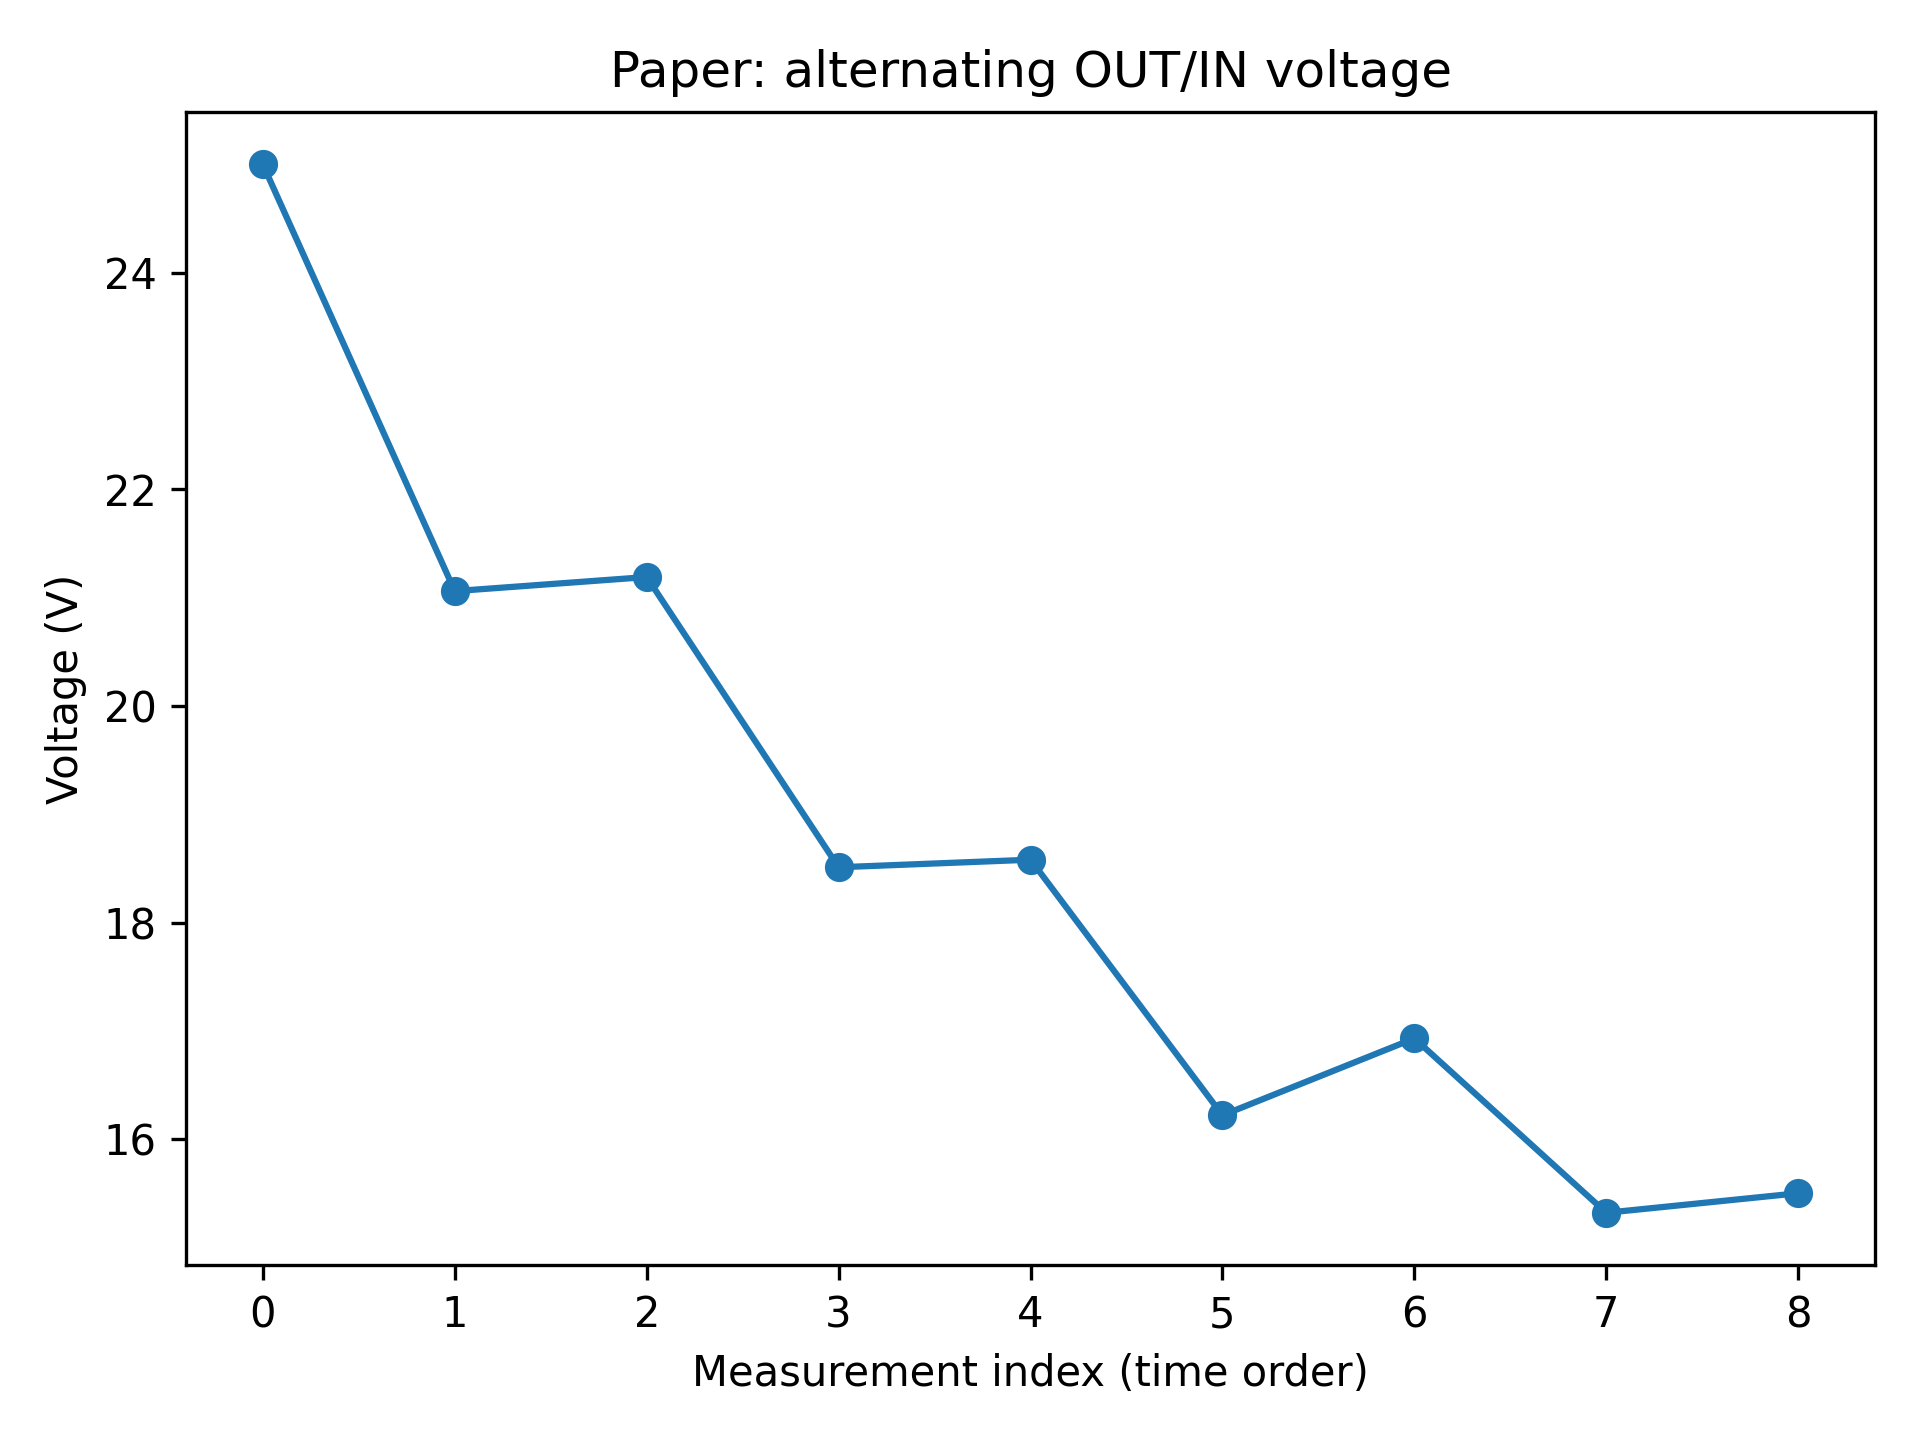
\includegraphics[width=0.70\linewidth]{PartB_paper.png}
\caption{\textbf{Part B -- Paper sequence.} Alternating OUT/IN voltages at fixed separation; IN values are generally lower, consistent with \(\kappa>1\).}
\label{fig:paper_seq}
\end{figure}

\begin{figure}[htbp]
\centering
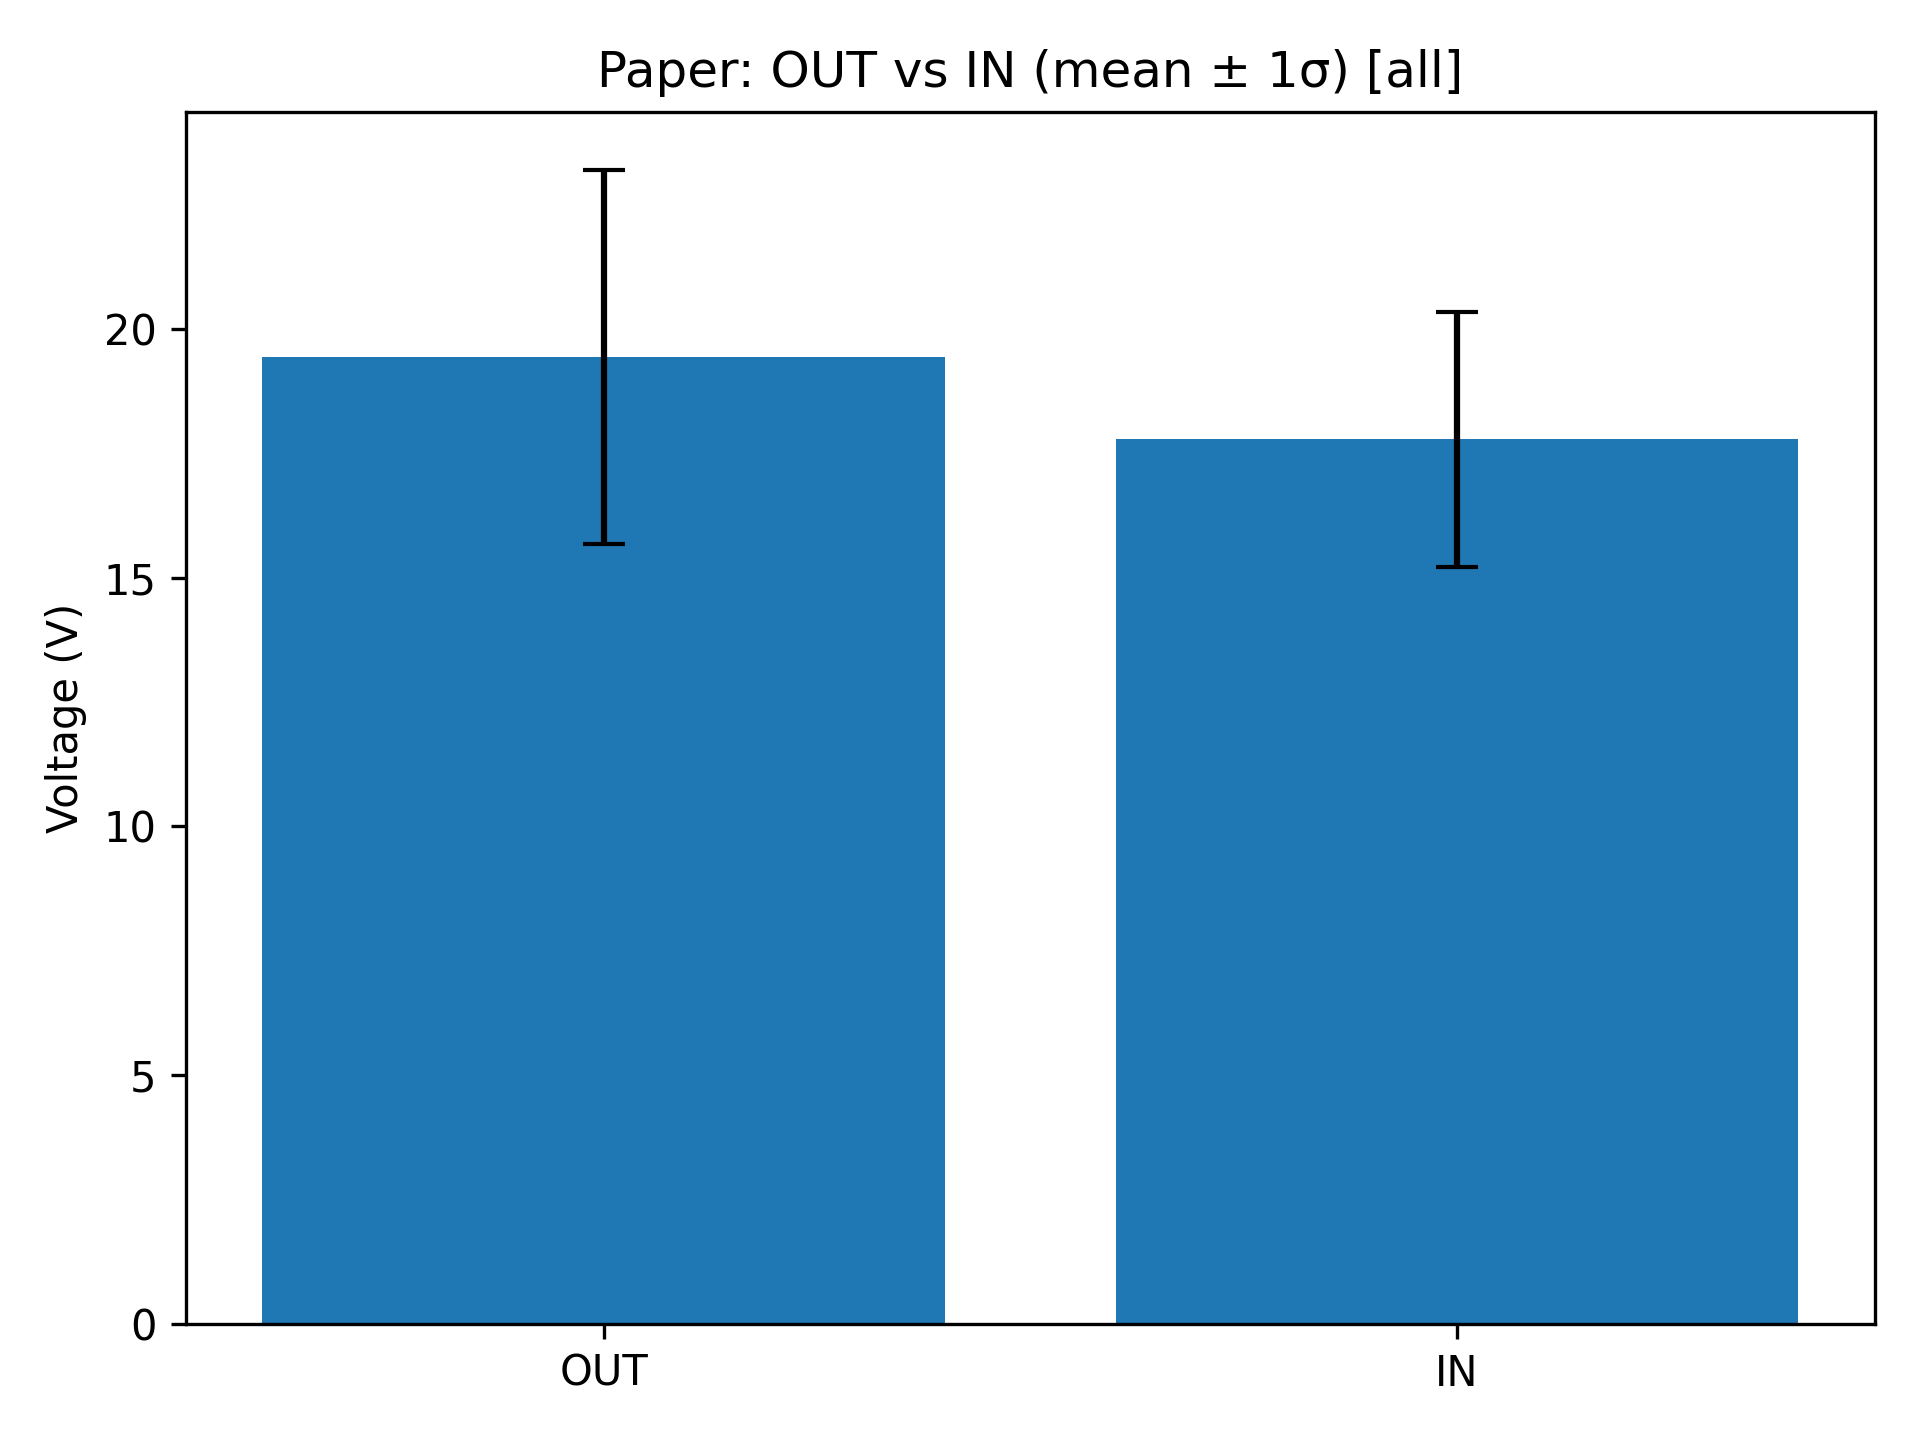
\includegraphics[width=0.58\linewidth]{PartB_OUTIN_bars_paper_all.png}
\caption{\textbf{Part B -- Paper OUT/IN comparison.} Mean \(\pm\) SD for OUT and IN; \(\kappa\) and \(\sigma_\kappa\) are evaluated via \cref{eq:kappa_formula}.}
\label{fig:paper_bars}
\end{figure}
\FloatBarrier

\paragraph{Plastic.}
The plastic sequence (\cref{fig:plastic_seq}) shows a strong early-time decrease upon insertion followed by large drift and even polarity reversal, indicating violation of the fixed-\(Q\) condition. Using the full series yields \(\mu_{\text{out}}=\SI{5.97}{V}\), \(\sigma_{\text{out}}=\SI{17.06}{V}\), \(\mu_{\text{in}}=\SI{1.28}{V}\), \(\sigma_{\text{in}}=\SI{16.39}{V}\), hence \(\kappa_{\text{plastic}}\approx 4.66\) with \(\sigma_\kappa\approx 61\) (uninformative). Restricting to only the first few stable OUT/IN pairs (not shown in figures) gives \(\kappa\sim 2\) but still with large uncertainty. The sequence and condensed comparison are shown in \cref{fig:plastic_seq,fig:plastic_bars}.

\begin{figure}[htbp]
\centering
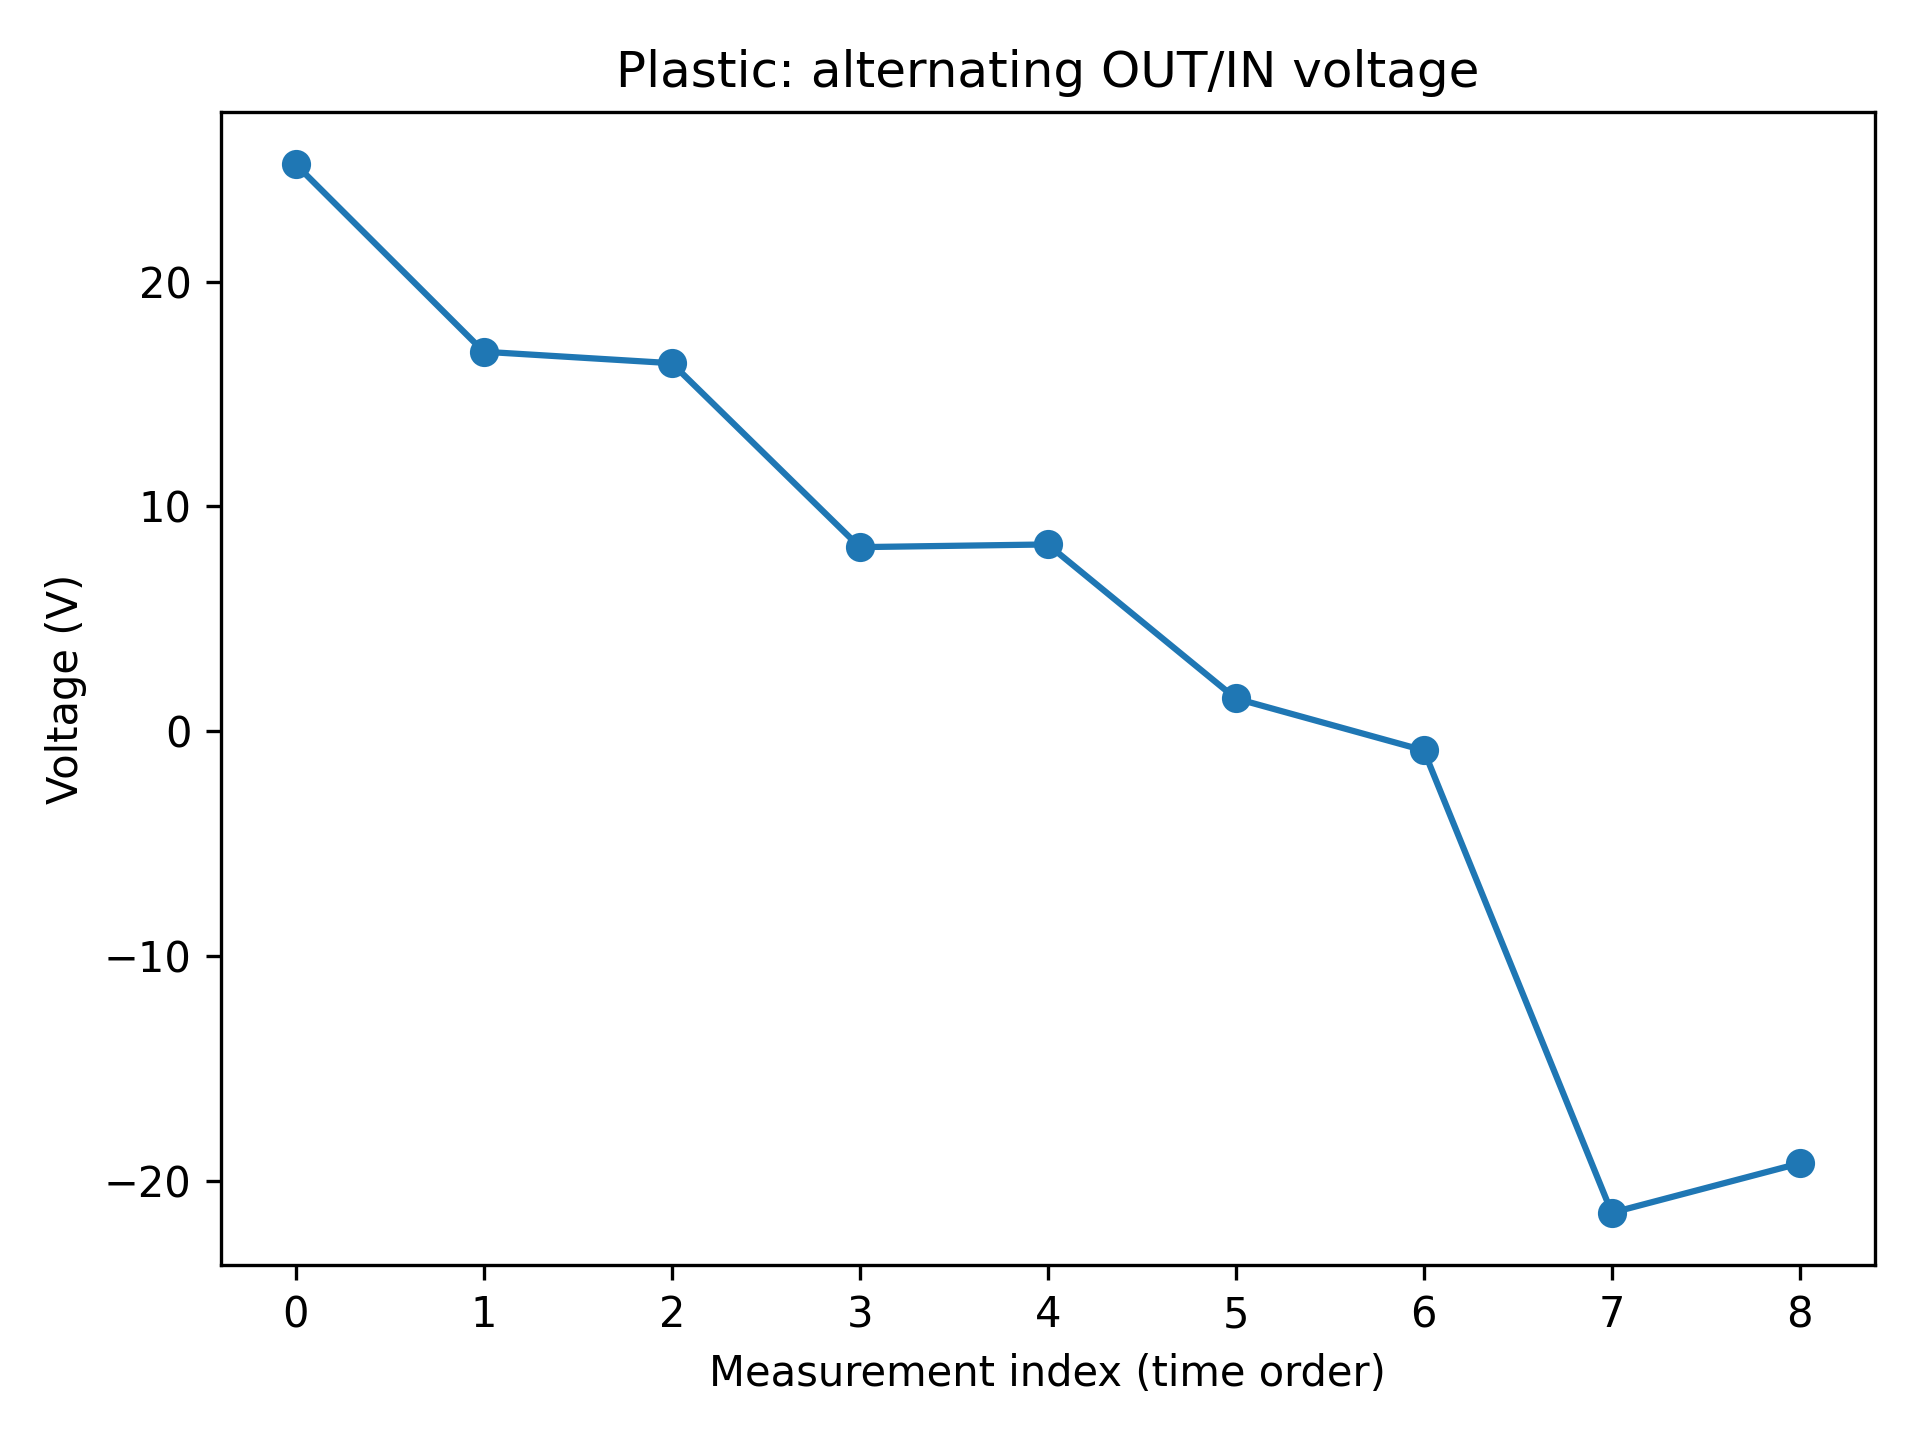
\includegraphics[width=0.70\linewidth]{PartB_plastic.png}
\caption{\textbf{Part B -- Plastic sequence.} Early-time response consistent with \(\kappa>1\); late-time drift dominates the uncertainty budget.}
\label{fig:plastic_seq}
\end{figure}

\begin{figure}[htbp]
\centering
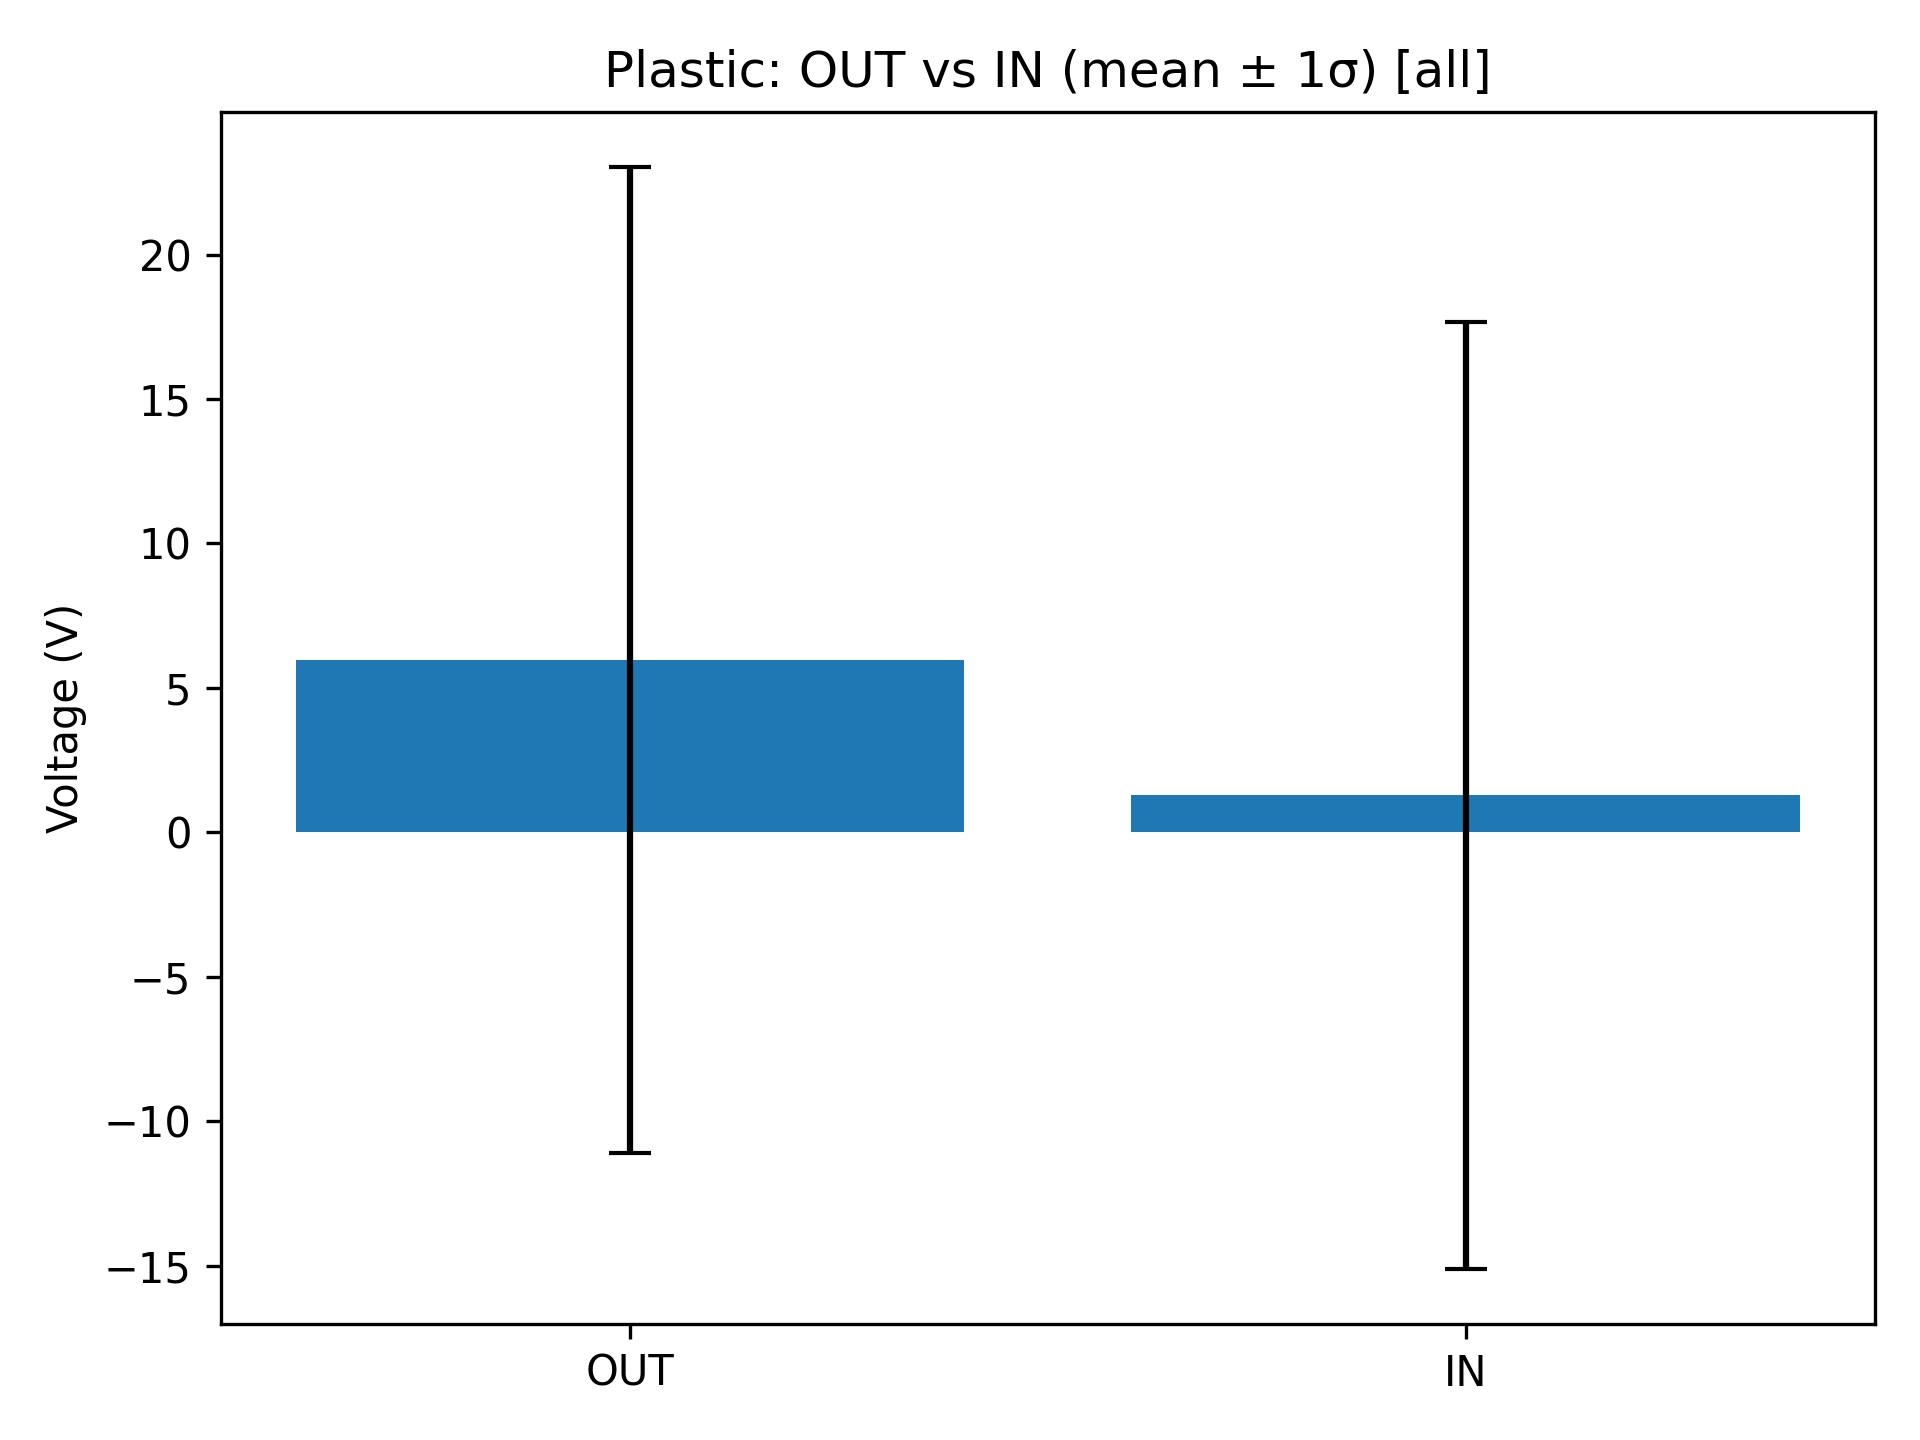
\includegraphics[width=0.58\linewidth]{PartB_OUTIN_bars_plastic_all.png}
\caption{\textbf{Part B -- Plastic OUT/IN comparison.} Mean \(\pm\) SD voltages; large error bars reflect charge leakage and drift.}
\label{fig:plastic_bars}
\end{figure}
\FloatBarrier

\paragraph{Glass.}
For glass, we obtain \(\mu_{\text{out}}=\SI{23.37}{V}\), \(\sigma_{\text{out}}=\SI{4.17}{V}\); \(\mu_{\text{in}}=\SI{27.77}{V}\), \(\sigma_{\text{in}}=\SI{2.76}{V}\), giving \(\kappa_{\text{glass}}=0.84\pm0.17\). Because \(\kappa<1\) is unphysical for an ideal insertion at fixed \(Q\), this indicates substantial discharge during the longer handling time. The alternating series and condensed comparison are shown in \cref{fig:glass_seq,fig:glass_bars}.

\begin{figure}[htbp]
\centering
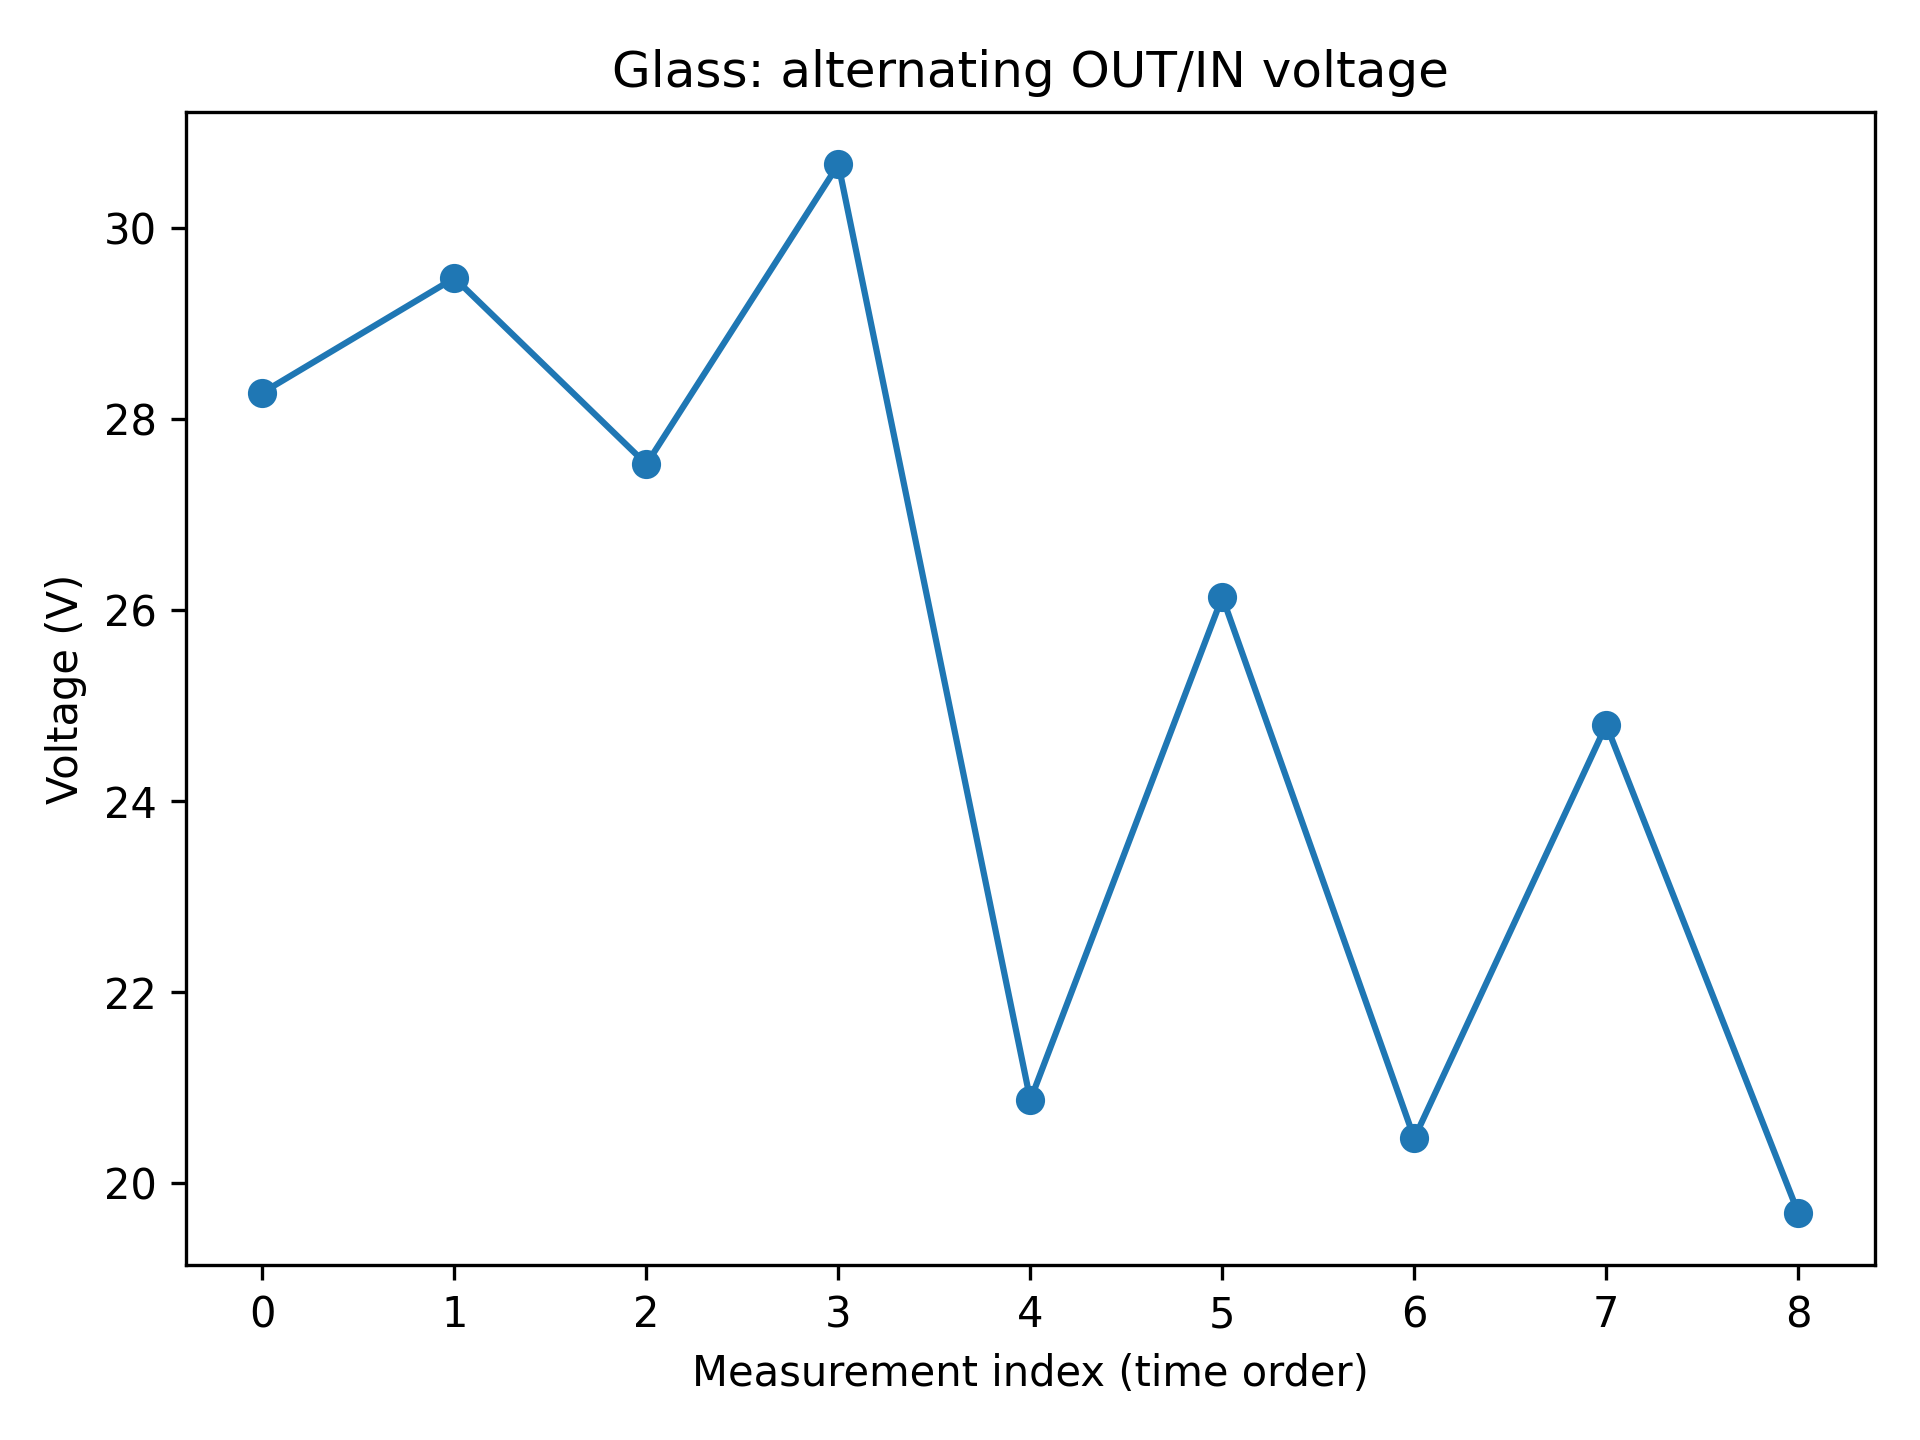
\includegraphics[width=0.70\linewidth]{PartB_glass.png}
\caption{\textbf{Part B -- Glass sequence.} Scatter and periods with IN \(>\) OUT indicate loss of charge during insertion.}
\label{fig:glass_seq}
\end{figure}

\begin{figure}[htbp]
\centering
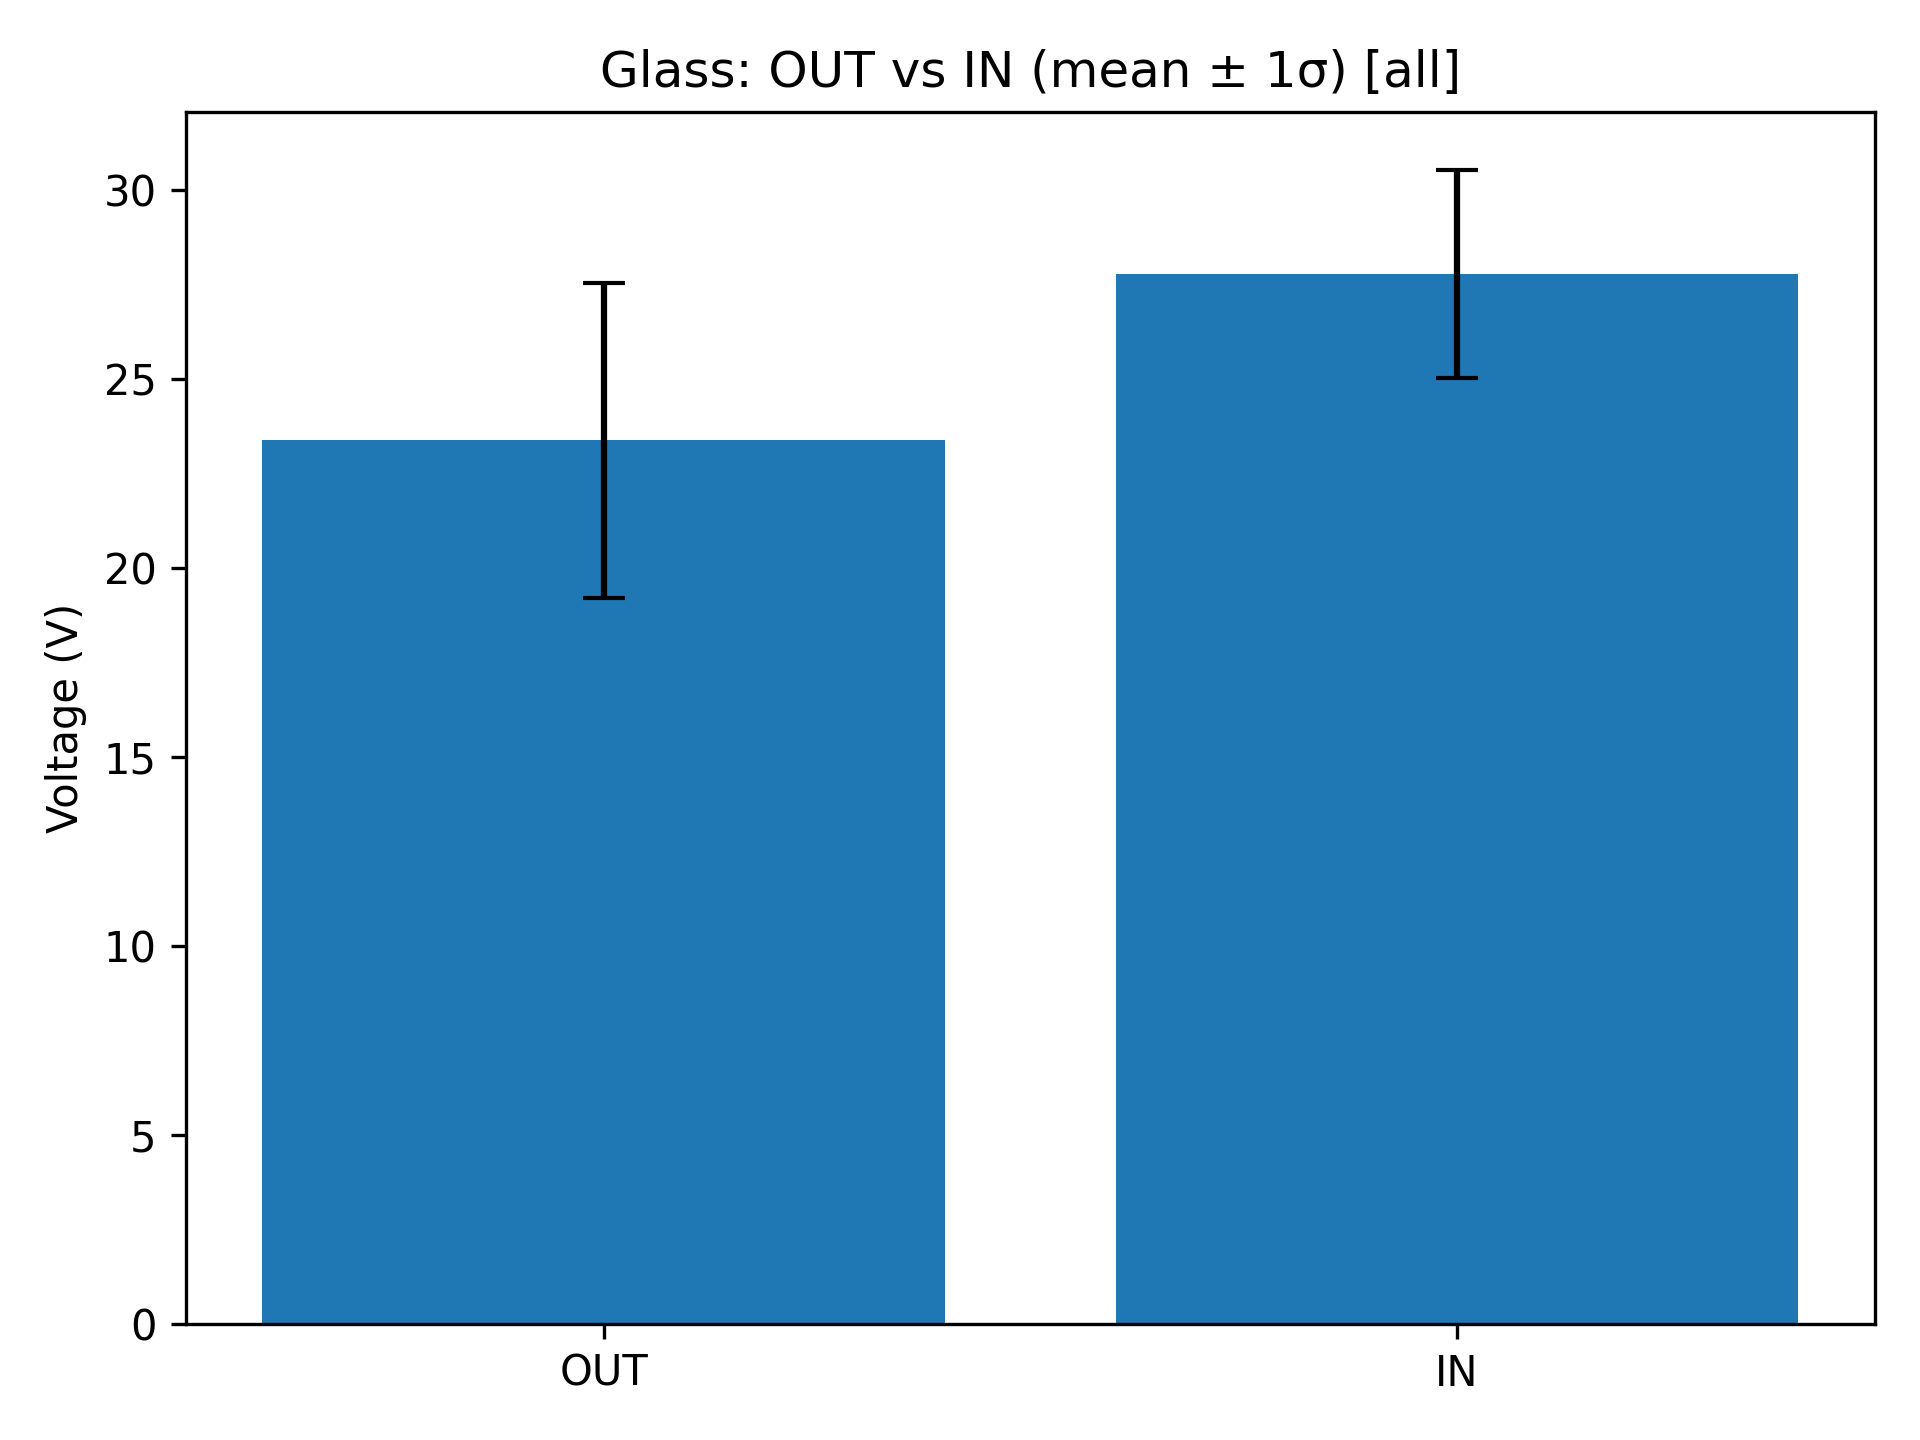
\includegraphics[width=0.58\linewidth]{PartB_OUTIN_bars_glass_all.png}
\caption{\textbf{Part B -- Glass OUT/IN comparison.} Mean \(\pm\) SD voltages; the apparent \(\kappa<1\) arises from leakage that violates the constant-\(Q\) assumption.}
\label{fig:glass_bars}
\end{figure}
\FloatBarrier


% ---------------- CONCLUSION ----------------
\section{Conclusion and Discussion}
The results confirm that the observed voltage across an isolated parallel-plate capacitor increases with plate separation according to \(V=Q/(\kappa\varepsilon_0A/d+C_{\mathrm{sys}})\).  
From the limiting-case analysis, the stored charge and system capacitance were
\(Q=(1.34\pm0.03)\times10^{-9}\,\mathrm{C}\) and
\(C_{\mathrm{sys}}=(3.24\pm0.14)\times10^{-11}\,\mathrm{F}\).
The inclusion of \(C_{\mathrm{sys}}\) is essential: without it the \(V\)–\(d\) relation would be linear, contradicting the observed saturation at large separations.
Residuals show random scatter, indicating that measurement noise rather than model deficiency limits the accuracy; the propagated-parameter band embraces essentially all points.

Insertion of dielectric materials reduced the measured voltage in most cases, supporting \(V_{\mathrm{in}}=V_{\mathrm{out}}/\kappa\).  
Paper produced a plausible \(\kappa\) near 1.1; plastic and glass data were corrupted by leakage and drift but qualitatively exhibit the same tendency.  
Experimental uncertainties arise mainly from leakage currents, humidity, operator proximity, and slow dielectric insertion.  
Reducing these effects would require shielding, faster data acquisition, and automated plate control.

% ---------------- REMARKS ----------------
\section{Remarks}
The main limitation of this experiment came from systematic errors such as charge leakage and small variations in the system capacitance \(C_{\mathrm{sys}}\) due to cable motion and operator proximity. These effects caused slow voltage drift, especially in the dielectric trials. Future improvements could include using simple shielding, recording each point promptly after charging, and securing plate alignment to reduce such systematic uncertainties.


\section*{Independent Writing Statement}
\emph{Experiment was performed jointly with Yifan Li, but this report was written independently to demonstrate individual understanding.}

\begin{thebibliography}{1}
\bibitem{manual}
Department Physics Laboratory, \emph{\ManualTitle}. 
\end{thebibliography}

\end{document}
